


\chapter{Cavitation of Water: 40\%}\label{ch:water_cavitation_char}


\section{Introduction}


Need to characterise the water sample.

Use of dirty water out of acceptance that characterisation required in any event.

To characterise we use knowledge of how oscillations are measured with ultrasound.
This is an inference problem.
We are fitting a model of the oscillations to the acquired data.
Need to be careful not to have a model that can fit anything.


\subsection{The Bayesian Approach}
Probability distributions can be used to represent our knowledge of the world.
For example, the value of a  experimentally obtained variable will in general
fluctuate around its average.  
If different runs of the experiment are independent
then the  distribution of obtained values fully describes the experiment.

What is learned from a given experiment is then characterised with how the probability distributions
that represent our knowledge change.
If a hypothesis, $\H$, is that a set of experimental data, $\vx = \{x_n|n=1,\ldots,N\}$, should conform to a model with a set of parameters, $\vw = \{w_i| i=1,\ldots,I\}$,
then our full knowledge of the system is given by the joint probability distribution
\begin{align}
  P\lr{\vx,\vw,\H}.
  \label{eqn:fullJointDist}
\end{align}
Of greater importance than \eqnref{fullJointDist}, however,
is to determine how our knowledge of the model changes when we collect the experimental data.
This can be found from  \eqnref{fullJointDist} by splitting the joint distribution into its conditional probabilities.
\begin{align}
  P\lr{\vx,\vw,\H} = P\lr{\vw|\vx,\H}P\lr{\vx|\H}
  =  P\lr{\vx|\vw,\H} P\lr{\vw|\H}.
\end{align}
from which it follows that 
\begin{align}
   P\lr{\vw|\vx,\H} =  \frac{P\lr{\vw|\vw,\H} P\lr{\vw|\H}}{P\lr{\vx|\H}}.
  \label{eqn:BayesTheorem}
\end{align}
Equation \Eqnref{BayesTheorem} is Bayes Theorem.
It states that the probability of the model's parameters, {\em given the data},
can be determined from the probability of the data when the parameters are known, and the a  probability of parameters {\em before the data was known}.
It describes exactly the process of inference.

The term $P\lr{\vx|\vw,\H}$ is the likelihood function.
It evaluates the degree to which the model with a given set of parameters agrees with the experimental data.
If it is assumed that every data point is independent, and that each datum should agree with the prediction of the model, $t_n$, 
to within Gaussian noise
then the likelihood function would be,
\begin{align}
  P\lr{\vx|\vw,\H} = \prod_{n=1}^N \sqrt{\frac{\gamma}{2\pi}}e^{-0.5\gamma\lr{x_n-t_n}^2}.
\end{align}
The variable $\gamma$ is the precision - the inverse of the variance - and is one of the set $\{w_i\}$.

The term $P\lr{\vw|\H}$ in \eqnref{BayesTheorem} is independent of the experimental data $\{x_n\}$.  
It  represents our knowledge of the parameters before the experiment was carried out.
It could be that the parameters are already known to great precision - 
in which case the probability distribution would tend towards a delta function.
Alternatively, it could that the a priori knowledge of the precision, say, 
does not expend beyond the requirement that the precision is positive definite.
In this case the prior distribution would be represented by a scale invariant positive definite distribution.
One such example is the Gamma distribution,
\begin{align}
  P(\gamma|s,c) = \frac{1}{\Gamma(s)c}\lr{\frac{x}{s}}^{c-1}\exp\lr{-\frac{x}{s}},
\label{eqn:Gamma}
\end{align}
in the limit such that $sc = 1$ and $c\rightarrow 0$ \cite{MacKay2003}.

The hypothesis, $\H$,  encompasses all of the assumptions that go into the inference.
These include the choice of the model that is fitted to the data, 
the prior probabilities assigned to the model variables and the 
the noise model described by the likelihood function.
These assumptions are inevitable - they reflect our uncertainty 
 prompts the experiment in the first place.
However, 
since many different hypotheses can be dreamed up,
it is important to be able to be able to evaluate how each is supported by the experimental data.
For this, Bayes Theorem can be applied a second time:
the probability of the hypothesis, given the data, is
\begin{align}
P\lr{\H | \vx } = \frac{P\lr{\vx|H}P\lr{\H}}{P\lr{\vx}}.
\label{eqn:BayesHyp}
\end{align}
Since the probability of the data, $P\lr{\vx}$, 
is independent of the hypothesis
it can be eliminated when comparing two hypotheses, $\H_1$ and $\H_2$,
\begin{align}
\frac{P\lr{\H_1 | \vx }}{P\lr{\H_2 | \vx }} = \frac{P\lr{\vx|\H_1}}{P\lr{\vx|\H_1}}\frac{P\lr{\H_2}}{P\lr{\H_2}}.
\label{eqn:ModelCmp}
\end{align}
The second of the ratios on the right-hand-side of \eqnref{ModelCmp}
give an opportunity, if desired, to prefer one model over another irrespectively of any data collected.
The first quotient is determined from the experimental data.
The term $P\lr{\vx|\H}$ is called the evidence and it is the partition function of  \eqnref{BayesHyp}.

A model that is highly constrained will be inflexible in the range of predictions it can make,
whereas a model that has many free parameters will be able to predict a vast number of possible outcomes.
The more constrained model will therefore have a smaller set of likely outcomes,
but each of these will have a much greater probability than the many possible outcomes of the less constrained model.
The right-hand-side of \eqnref{ModelCmp} therefore directly and quantitively embodies Occan's razor,
the rule of thumb that states that `simpler' models should be favoured over more complicated models.
For a more detailed discussion of model comparison and Occan's razor see \cite[Chapter 28]{Mackay2003}.

To evaluate the evidence the numerator in equation \eqnref{BayesTheorem} must be integrated over the entire parameter space,
\begin{align}
  P\lr{\vx|\H} = \int_\vw d\vw P\lr{\vw|\vw,\H} P\lr{\vw|\H}
\end{align}
In general this cannot be done analytically.
However, it is often the case that the probability density tightly peaked about the maximum.
In this case the evidence may be evaluated by approximating the peak with a Gaussian, which can be integrated.
This is the saddle point approximation.
Expanding the logarithm of the  unnormalised probability distribution, $P^\ast$, 
around the maximum, $\vx_0$,
gives
\eq{
  \ln P^\ast = \ln P^\ast(\vx_0) - \frac{1}{2}\lr{\vx-\vx_0}^T \vA\lr{\vx-\vx_0 }
}
where 
\eq{
\vA = A_{ij} = \frac{\d^2}{\d x_i\d x_j} \ln P^\ast(\vx_0)
}
is the Hessian matrix.
The right-hand-side of equation \eqnref{BayesTheorem}  is therefore approximated by the multidimensional Gaussian
\begin{align}
   P\lr{\vw|\vx,\H} = P^\ast(\vx_0) \exp \lr{- \frac{1}{2}\lr{\vx-\vx_0}^T \vA\lr{\vx-\vx_0 }}
\end{align}
for which the normalisation constant, the evidence, is 
\begin{align}
   P^\ast(\vx_0) \sqrt{\frac{\lr{2\pi}^K}{\det \vA}}
\end{align}

\section{First inference}

Make a first inference,
can then use model comparison to improve if needed.

\subsection{Assumptions}

A simple (if slightly optimistic) model for the pulsations of the bubble 
is constructed by  assuming
\nlist{
\item the pressure wave emanates from a bubble (or set of mono-disperse bubbles).
  The free parameter being the equilibrium bubble radius.
\item the pressure wave is \unit{$\frac{1}{2}$}\mega\hertz\ sinusoid of 13 cycles that is truncated by a cosine function.
  The free parameters being the peak amplitude, the fraction of the wave truncated by the sinusoid, 
  and the offset of the sinusoid in time.
\item The noise is Gaussian white noise with a standard deviation that is modelled.
\item The voltage generated by the transducer is equal to the far-field pressure to within a (modelled)  multiplicative factor.
  (I.e. assuming infinite bandwidth of the transducer and receive electronics).  
}

The likelihood that we maximise is that
\eql{
  P\lr{\vx|\vw,\H}  =  \prod_{t=0}^T\G(x_t; \mu_t, \gamma)
}{likelihoodFirst}
where 
\eq{
  \G(x;\mu,\gamma) =\sqrt{\frac{\gamma}{2\pi}}e^{-0.5\gamma\lr{x-\mu}^2}
}
is a Gaussian distribution of mean $\mu$ and precision  $\gamma$.
Each data point recorded is denoted $x_t$ and the modelled point (given the parameters) the mean  $\mu_t$.
The bubble radius, noise precision, pressure and offset and truncation ratio are all positive quantities which we model with Gamma distributions.
However, to enforce positivity during the iterative numerical updates 
we reparameterise the gamma distribution of equation \eqnref{Gamma} such that $l = ln(x)$.
If follows that
\begin{align}
  P(l) = P(x(l))\abs{\frac{\partial x}{\partial l}} = \frac{1}{\Gamma(c)}\lr{\frac{x(l)}{s}}^c\exp\lr{-x(l)/s}.
\label{eqn:logGamma}
\end{align}
For the time being we assume that the priors are non-informative, such that $sc = 1$ and $c\rightarrow 0$,
from which it follows that \eqnref{logGamma} is flat.
To find the most likely parameters of the model, 
equation \eqnref{BayesTheorem} tells us that in this case we must  maximise the likelihood.



Since the model is non-linear,
maximising the likelihood with a gradient approach is impossible.
Therefore, to maximise \eqnref{likelihoodFirst}
we use the simplex minimisation of Nelder and Mead\cite{Nelder1965}
to minimise the negative of the log likelihood.
The implemenation that is used is that of the Gnu Scientific Library.

%\subsubsection{Simplex Approach}
The simplex approach of Nelder and Mead\cite{Nelder1965} starts from an initial position $\vx_i$ and
constructs a further $N$ points from a initial step-size in each dimension that is provided on initialisation.
At each iteration a new simplex is constructed that is closer to a minimum.

One slight complication with the simplex approach is in approximating the Hessian matrix
that is required for model comparison.
Since (and quite deliberatly)
this minimisation method does not rely on derivatives,
no Hessian matrix can be directly evaluated.
An approach for doing this was provided in  Nelder and Mead's original article\cite{Nelder1965}.
%Once the simplex has converged, 
%a basis may be chosen from the $n+1$ points, such that the points are
%\begin{align}
%(0,0, \ldots, 0)\\
%(1,0, \ldots, 0)\\
%(0,1, \ldots, 0)\\
%\hdots \\
%(0,0, \ldots, 1)\\
%\end{align}
%so that in vicinity of minimum surface can be approximated to quadratic precision according to 
%\begin{align}
%   y =  a_0 + 2  a\cdot x  +  x^\prime B x
%\end{align}



\subsubsection{Results}



\begin{figure}[t]%
  \centering
  \subfloat[Bubble radius:  \unit{0.4107}\micro\metre]{
    \label{fig:plot_bubble_fit_108_150:first}
    % GNUPLOT: LaTeX picture with Postscript
\begingroup
  \makeatletter
  \providecommand\color[2][]{%
    \GenericError{(gnuplot) \space\space\space\@spaces}{%
      Package color not loaded in conjunction with
      terminal option `colourtext'%
    }{See the gnuplot documentation for explanation.%
    }{Either use 'blacktext' in gnuplot or load the package
      color.sty in LaTeX.}%
    \renewcommand\color[2][]{}%
  }%
  \providecommand\includegraphics[2][]{%
    \GenericError{(gnuplot) \space\space\space\@spaces}{%
      Package graphicx or graphics not loaded%
    }{See the gnuplot documentation for explanation.%
    }{The gnuplot epslatex terminal needs graphicx.sty or graphics.sty.}%
    \renewcommand\includegraphics[2][]{}%
  }%
  \providecommand\rotatebox[2]{#2}%
  \@ifundefined{ifGPcolor}{%
    \newif\ifGPcolor
    \GPcolortrue
  }{}%
  \@ifundefined{ifGPblacktext}{%
    \newif\ifGPblacktext
    \GPblacktexttrue
  }{}%
  % define a \g@addto@macro without @ in the name:
  \let\gplgaddtomacro\g@addto@macro
  % define empty templates for all commands taking text:
  \gdef\gplbacktext{}%
  \gdef\gplfronttext{}%
  \makeatother
  \ifGPblacktext
    % no textcolor at all
    \def\colorrgb#1{}%
    \def\colorgray#1{}%
  \else
    % gray or color?
    \ifGPcolor
      \def\colorrgb#1{\color[rgb]{#1}}%
      \def\colorgray#1{\color[gray]{#1}}%
      \expandafter\def\csname LTw\endcsname{\color{white}}%
      \expandafter\def\csname LTb\endcsname{\color{black}}%
      \expandafter\def\csname LTa\endcsname{\color{black}}%
      \expandafter\def\csname LT0\endcsname{\color[rgb]{1,0,0}}%
      \expandafter\def\csname LT1\endcsname{\color[rgb]{0,1,0}}%
      \expandafter\def\csname LT2\endcsname{\color[rgb]{0,0,1}}%
      \expandafter\def\csname LT3\endcsname{\color[rgb]{1,0,1}}%
      \expandafter\def\csname LT4\endcsname{\color[rgb]{0,1,1}}%
      \expandafter\def\csname LT5\endcsname{\color[rgb]{1,1,0}}%
      \expandafter\def\csname LT6\endcsname{\color[rgb]{0,0,0}}%
      \expandafter\def\csname LT7\endcsname{\color[rgb]{1,0.3,0}}%
      \expandafter\def\csname LT8\endcsname{\color[rgb]{0.5,0.5,0.5}}%
    \else
      % gray
      \def\colorrgb#1{\color{black}}%
      \def\colorgray#1{\color[gray]{#1}}%
      \expandafter\def\csname LTw\endcsname{\color{white}}%
      \expandafter\def\csname LTb\endcsname{\color{black}}%
      \expandafter\def\csname LTa\endcsname{\color{black}}%
      \expandafter\def\csname LT0\endcsname{\color{black}}%
      \expandafter\def\csname LT1\endcsname{\color{black}}%
      \expandafter\def\csname LT2\endcsname{\color{black}}%
      \expandafter\def\csname LT3\endcsname{\color{black}}%
      \expandafter\def\csname LT4\endcsname{\color{black}}%
      \expandafter\def\csname LT5\endcsname{\color{black}}%
      \expandafter\def\csname LT6\endcsname{\color{black}}%
      \expandafter\def\csname LT7\endcsname{\color{black}}%
      \expandafter\def\csname LT8\endcsname{\color{black}}%
    \fi
  \fi
  \setlength{\unitlength}{0.0500bp}%
  \begin{picture}(5760.00,2520.00)%
    \gplgaddtomacro\gplbacktext{%
      \csname LTb\endcsname%
      \put(-119,865){\makebox(0,0)[r]{\strut{}-0.2}}%
      \put(-119,1187){\makebox(0,0)[r]{\strut{}-0.1}}%
      \put(-119,1509){\makebox(0,0)[r]{\strut{} 0}}%
      \put(-119,1832){\makebox(0,0)[r]{\strut{} 0.1}}%
      \put(-119,2154){\makebox(0,0)[r]{\strut{} 0.2}}%
      \put(-119,2476){\makebox(0,0)[r]{\strut{} 0.3}}%
      \put(13,484){\makebox(0,0){\strut{} 0}}%
      \put(832,484){\makebox(0,0){\strut{} 5}}%
      \put(1651,484){\makebox(0,0){\strut{} 10}}%
      \put(2470,484){\makebox(0,0){\strut{} 15}}%
      \put(3289,484){\makebox(0,0){\strut{} 20}}%
      \put(4108,484){\makebox(0,0){\strut{} 25}}%
      \put(4927,484){\makebox(0,0){\strut{} 30}}%
      \put(5746,484){\makebox(0,0){\strut{} 35}}%
      \put(-889,1590){\rotatebox{-270}{\makebox(0,0){\strut{}voltage (V)}}}%
      \put(2879,154){\makebox(0,0){\strut{}time ($\mu$ s)}}%
    }%
    \gplgaddtomacro\gplfronttext{%
      \csname LTb\endcsname%
      \put(5261,2303){\makebox(0,0){\footnotesize {raw}} }%
      \csname LTb\endcsname%
      \put(5261,2083){\makebox(0,0){\footnotesize {1-$\sigma$}}}%
      \csname LTb\endcsname%
      \put(5261,1863){\makebox(0,0){\footnotesize {fit}}}%
    }%
    \gplbacktext
    \put(0,0){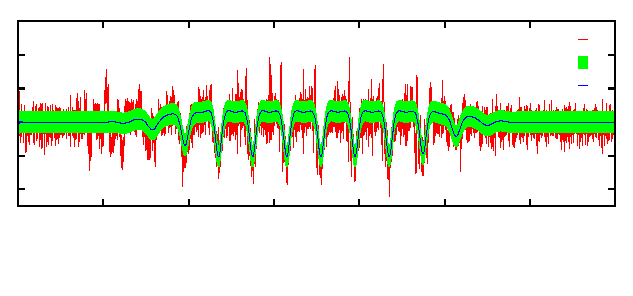
\includegraphics{plot_bubble_fit_108_150}}%
    \gplfronttext
  \end{picture}%
\endgroup
}\\
  \subfloat[Bubble radius:  \unit{0.1064}\micro\metre]{
    \label{fig:plot_bubble_fit_108_150:second}
    % GNUPLOT: LaTeX picture with Postscript
\begingroup
  \makeatletter
  \providecommand\color[2][]{%
    \GenericError{(gnuplot) \space\space\space\@spaces}{%
      Package color not loaded in conjunction with
      terminal option `colourtext'%
    }{See the gnuplot documentation for explanation.%
    }{Either use 'blacktext' in gnuplot or load the package
      color.sty in LaTeX.}%
    \renewcommand\color[2][]{}%
  }%
  \providecommand\includegraphics[2][]{%
    \GenericError{(gnuplot) \space\space\space\@spaces}{%
      Package graphicx or graphics not loaded%
    }{See the gnuplot documentation for explanation.%
    }{The gnuplot epslatex terminal needs graphicx.sty or graphics.sty.}%
    \renewcommand\includegraphics[2][]{}%
  }%
  \providecommand\rotatebox[2]{#2}%
  \@ifundefined{ifGPcolor}{%
    \newif\ifGPcolor
    \GPcolortrue
  }{}%
  \@ifundefined{ifGPblacktext}{%
    \newif\ifGPblacktext
    \GPblacktexttrue
  }{}%
  % define a \g@addto@macro without @ in the name:
  \let\gplgaddtomacro\g@addto@macro
  % define empty templates for all commands taking text:
  \gdef\gplbacktext{}%
  \gdef\gplfronttext{}%
  \makeatother
  \ifGPblacktext
    % no textcolor at all
    \def\colorrgb#1{}%
    \def\colorgray#1{}%
  \else
    % gray or color?
    \ifGPcolor
      \def\colorrgb#1{\color[rgb]{#1}}%
      \def\colorgray#1{\color[gray]{#1}}%
      \expandafter\def\csname LTw\endcsname{\color{white}}%
      \expandafter\def\csname LTb\endcsname{\color{black}}%
      \expandafter\def\csname LTa\endcsname{\color{black}}%
      \expandafter\def\csname LT0\endcsname{\color[rgb]{1,0,0}}%
      \expandafter\def\csname LT1\endcsname{\color[rgb]{0,1,0}}%
      \expandafter\def\csname LT2\endcsname{\color[rgb]{0,0,1}}%
      \expandafter\def\csname LT3\endcsname{\color[rgb]{1,0,1}}%
      \expandafter\def\csname LT4\endcsname{\color[rgb]{0,1,1}}%
      \expandafter\def\csname LT5\endcsname{\color[rgb]{1,1,0}}%
      \expandafter\def\csname LT6\endcsname{\color[rgb]{0,0,0}}%
      \expandafter\def\csname LT7\endcsname{\color[rgb]{1,0.3,0}}%
      \expandafter\def\csname LT8\endcsname{\color[rgb]{0.5,0.5,0.5}}%
    \else
      % gray
      \def\colorrgb#1{\color{black}}%
      \def\colorgray#1{\color[gray]{#1}}%
      \expandafter\def\csname LTw\endcsname{\color{white}}%
      \expandafter\def\csname LTb\endcsname{\color{black}}%
      \expandafter\def\csname LTa\endcsname{\color{black}}%
      \expandafter\def\csname LT0\endcsname{\color{black}}%
      \expandafter\def\csname LT1\endcsname{\color{black}}%
      \expandafter\def\csname LT2\endcsname{\color{black}}%
      \expandafter\def\csname LT3\endcsname{\color{black}}%
      \expandafter\def\csname LT4\endcsname{\color{black}}%
      \expandafter\def\csname LT5\endcsname{\color{black}}%
      \expandafter\def\csname LT6\endcsname{\color{black}}%
      \expandafter\def\csname LT7\endcsname{\color{black}}%
      \expandafter\def\csname LT8\endcsname{\color{black}}%
    \fi
  \fi
  \setlength{\unitlength}{0.0500bp}%
  \begin{picture}(5760.00,2520.00)%
    \gplgaddtomacro\gplbacktext{%
      \csname LTb\endcsname%
      \put(-119,865){\makebox(0,0)[r]{\strut{}-0.2}}%
      \put(-119,1187){\makebox(0,0)[r]{\strut{}-0.1}}%
      \put(-119,1509){\makebox(0,0)[r]{\strut{} 0}}%
      \put(-119,1832){\makebox(0,0)[r]{\strut{} 0.1}}%
      \put(-119,2154){\makebox(0,0)[r]{\strut{} 0.2}}%
      \put(-119,2476){\makebox(0,0)[r]{\strut{} 0.3}}%
      \put(13,484){\makebox(0,0){\strut{} 0}}%
      \put(832,484){\makebox(0,0){\strut{} 5}}%
      \put(1651,484){\makebox(0,0){\strut{} 10}}%
      \put(2470,484){\makebox(0,0){\strut{} 15}}%
      \put(3289,484){\makebox(0,0){\strut{} 20}}%
      \put(4108,484){\makebox(0,0){\strut{} 25}}%
      \put(4927,484){\makebox(0,0){\strut{} 30}}%
      \put(5746,484){\makebox(0,0){\strut{} 35}}%
      \put(-889,1590){\rotatebox{-270}{\makebox(0,0){\strut{}voltage (V)}}}%
      \put(2879,154){\makebox(0,0){\strut{}time ($\mu$ s)}}%
    }%
    \gplgaddtomacro\gplfronttext{%
      \csname LTb\endcsname%
      \put(5261,2303){\makebox(0,0){\footnotesize {raw}} }%
      \csname LTb\endcsname%
      \put(5261,2083){\makebox(0,0){\footnotesize {1-$\sigma$}}}%
      \csname LTb\endcsname%
      \put(5261,1863){\makebox(0,0){\footnotesize {fit}}}%
    }%
    \gplbacktext
    \put(0,0){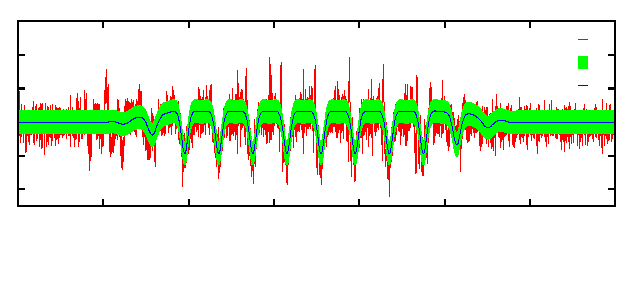
\includegraphics{plot_bubble_fit_108_150_b}}%
    \gplfronttext
  \end{picture}%
\endgroup
}\\
  \subfloat[Bubble radius:  \unit{0.2028}\micro\metre]{
    \label{fig:plot_bubble_fit_108_150:third}
    % GNUPLOT: LaTeX picture with Postscript
\begingroup
  \makeatletter
  \providecommand\color[2][]{%
    \GenericError{(gnuplot) \space\space\space\@spaces}{%
      Package color not loaded in conjunction with
      terminal option `colourtext'%
    }{See the gnuplot documentation for explanation.%
    }{Either use 'blacktext' in gnuplot or load the package
      color.sty in LaTeX.}%
    \renewcommand\color[2][]{}%
  }%
  \providecommand\includegraphics[2][]{%
    \GenericError{(gnuplot) \space\space\space\@spaces}{%
      Package graphicx or graphics not loaded%
    }{See the gnuplot documentation for explanation.%
    }{The gnuplot epslatex terminal needs graphicx.sty or graphics.sty.}%
    \renewcommand\includegraphics[2][]{}%
  }%
  \providecommand\rotatebox[2]{#2}%
  \@ifundefined{ifGPcolor}{%
    \newif\ifGPcolor
    \GPcolortrue
  }{}%
  \@ifundefined{ifGPblacktext}{%
    \newif\ifGPblacktext
    \GPblacktexttrue
  }{}%
  % define a \g@addto@macro without @ in the name:
  \let\gplgaddtomacro\g@addto@macro
  % define empty templates for all commands taking text:
  \gdef\gplbacktext{}%
  \gdef\gplfronttext{}%
  \makeatother
  \ifGPblacktext
    % no textcolor at all
    \def\colorrgb#1{}%
    \def\colorgray#1{}%
  \else
    % gray or color?
    \ifGPcolor
      \def\colorrgb#1{\color[rgb]{#1}}%
      \def\colorgray#1{\color[gray]{#1}}%
      \expandafter\def\csname LTw\endcsname{\color{white}}%
      \expandafter\def\csname LTb\endcsname{\color{black}}%
      \expandafter\def\csname LTa\endcsname{\color{black}}%
      \expandafter\def\csname LT0\endcsname{\color[rgb]{1,0,0}}%
      \expandafter\def\csname LT1\endcsname{\color[rgb]{0,1,0}}%
      \expandafter\def\csname LT2\endcsname{\color[rgb]{0,0,1}}%
      \expandafter\def\csname LT3\endcsname{\color[rgb]{1,0,1}}%
      \expandafter\def\csname LT4\endcsname{\color[rgb]{0,1,1}}%
      \expandafter\def\csname LT5\endcsname{\color[rgb]{1,1,0}}%
      \expandafter\def\csname LT6\endcsname{\color[rgb]{0,0,0}}%
      \expandafter\def\csname LT7\endcsname{\color[rgb]{1,0.3,0}}%
      \expandafter\def\csname LT8\endcsname{\color[rgb]{0.5,0.5,0.5}}%
    \else
      % gray
      \def\colorrgb#1{\color{black}}%
      \def\colorgray#1{\color[gray]{#1}}%
      \expandafter\def\csname LTw\endcsname{\color{white}}%
      \expandafter\def\csname LTb\endcsname{\color{black}}%
      \expandafter\def\csname LTa\endcsname{\color{black}}%
      \expandafter\def\csname LT0\endcsname{\color{black}}%
      \expandafter\def\csname LT1\endcsname{\color{black}}%
      \expandafter\def\csname LT2\endcsname{\color{black}}%
      \expandafter\def\csname LT3\endcsname{\color{black}}%
      \expandafter\def\csname LT4\endcsname{\color{black}}%
      \expandafter\def\csname LT5\endcsname{\color{black}}%
      \expandafter\def\csname LT6\endcsname{\color{black}}%
      \expandafter\def\csname LT7\endcsname{\color{black}}%
      \expandafter\def\csname LT8\endcsname{\color{black}}%
    \fi
  \fi
  \setlength{\unitlength}{0.0500bp}%
  \begin{picture}(5760.00,2520.00)%
    \gplgaddtomacro\gplbacktext{%
      \csname LTb\endcsname%
      \put(-119,865){\makebox(0,0)[r]{\strut{}-0.2}}%
      \put(-119,1187){\makebox(0,0)[r]{\strut{}-0.1}}%
      \put(-119,1509){\makebox(0,0)[r]{\strut{} 0}}%
      \put(-119,1832){\makebox(0,0)[r]{\strut{} 0.1}}%
      \put(-119,2154){\makebox(0,0)[r]{\strut{} 0.2}}%
      \put(-119,2476){\makebox(0,0)[r]{\strut{} 0.3}}%
      \put(13,484){\makebox(0,0){\strut{} 0}}%
      \put(832,484){\makebox(0,0){\strut{} 5}}%
      \put(1651,484){\makebox(0,0){\strut{} 10}}%
      \put(2470,484){\makebox(0,0){\strut{} 15}}%
      \put(3289,484){\makebox(0,0){\strut{} 20}}%
      \put(4108,484){\makebox(0,0){\strut{} 25}}%
      \put(4927,484){\makebox(0,0){\strut{} 30}}%
      \put(5746,484){\makebox(0,0){\strut{} 35}}%
      \put(-889,1590){\rotatebox{-270}{\makebox(0,0){\strut{}voltage (V)}}}%
      \put(2879,154){\makebox(0,0){\strut{}time ($\mu$ s)}}%
    }%
    \gplgaddtomacro\gplfronttext{%
      \csname LTb\endcsname%
      \put(5261,2303){\makebox(0,0){\footnotesize {raw}} }%
      \csname LTb\endcsname%
      \put(5261,2083){\makebox(0,0){\footnotesize {1-$\sigma$}}}%
      \csname LTb\endcsname%
      \put(5261,1863){\makebox(0,0){\footnotesize {fit}}}%
    }%
    \gplbacktext
    \put(0,0){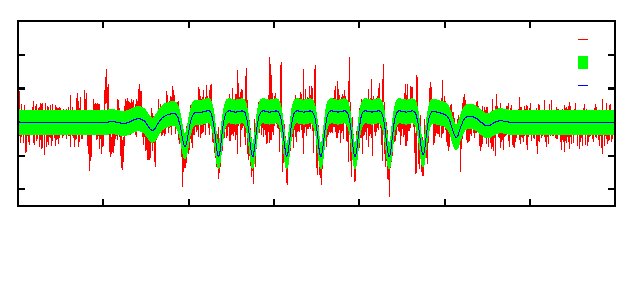
\includegraphics{plot_bubble_fit_108_150_c}}%
    \gplfronttext
  \end{picture}%
\endgroup
}
  \label{fig:plot_bubble_fit_108_150}
\caption{Voltage 0.108, 150}
\end{figure}


\ctable[cap     = Parameters for \figref{plot_bubble_fit_108_150:first} (RKM),
        caption = Parameters for \figref{plot_bubble_fit_108_150:first},
        label   = table:fit_108_150,
        pos   = h,
        %width = 0.6\textwidth,
        left
       ]
       {llcrccccc}
{
}{\FL
    &   Parameter      &  Initial 1 &Initial 2&Initial 3 & Fitted 1  &Fitted 2 &Fitted 3  &
    \ML
    &scale factor & 3000 & 3000  & 3000 & 345.7 & 5729 & 1472
    \NN
    &standard-deviation & \unit{0.03}\volt & \unit{0.03}\volt & \unit{0.03}\volt &  \unit{0.03034}\volt  & \unit{0.03371}\volt& \unit{0.03561}\volt& 
    \NN
    &bubble radius &\unit{0.5}\micro\metre   &\unit{1.3}\micro\metre&\unit{0.2}\micro\metre   & \unit{0.4107}\micro\metre & \unit{0.1064}\micro\metre&  \unit{0.2028}\micro\metre& 
    \NN
    &pulse amplitude&\unit{0.1}\mega\pascal &   \unit{0.1}\mega\pascal &   \unit{0.1}\mega\pascal  &      \unit{0.1290}\mega\pascal   &   \unit{0.3448}\mega\pascal     &  \unit{0.2185}\mega\pascal     & 
    \NN
    &pulse offset &\unit{29.2}\micro\second &   \unit{29.2}\micro\second &   \unit{29.2}\micro\second &      \unit{29.25}\micro\second   & \unit{29.24}\micro\second   &  \unit{29.25}\micro\second   &  
    \NN
    &pulse tempered ratio &0.5 &0.5 &0.5 & 0.53  & 0.40595  & 0.5189 &
    \NN
    &log (evidence) & & & & -18908.29097 & -19128.52276 &  -19209.08907
    \LL
}


\begin{figure}[t]%
  \centering
  \subfloat[1st pulse - 1000]{
    \label{fig:plot_bubble_fit_108_150_l:combo}
    % GNUPLOT: LaTeX picture with Postscript
\begingroup
  \makeatletter
  \providecommand\color[2][]{%
    \GenericError{(gnuplot) \space\space\space\@spaces}{%
      Package color not loaded in conjunction with
      terminal option `colourtext'%
    }{See the gnuplot documentation for explanation.%
    }{Either use 'blacktext' in gnuplot or load the package
      color.sty in LaTeX.}%
    \renewcommand\color[2][]{}%
  }%
  \providecommand\includegraphics[2][]{%
    \GenericError{(gnuplot) \space\space\space\@spaces}{%
      Package graphicx or graphics not loaded%
    }{See the gnuplot documentation for explanation.%
    }{The gnuplot epslatex terminal needs graphicx.sty or graphics.sty.}%
    \renewcommand\includegraphics[2][]{}%
  }%
  \providecommand\rotatebox[2]{#2}%
  \@ifundefined{ifGPcolor}{%
    \newif\ifGPcolor
    \GPcolortrue
  }{}%
  \@ifundefined{ifGPblacktext}{%
    \newif\ifGPblacktext
    \GPblacktexttrue
  }{}%
  % define a \g@addto@macro without @ in the name:
  \let\gplgaddtomacro\g@addto@macro
  % define empty templates for all commands taking text:
  \gdef\gplbacktext{}%
  \gdef\gplfronttext{}%
  \makeatother
  \ifGPblacktext
    % no textcolor at all
    \def\colorrgb#1{}%
    \def\colorgray#1{}%
  \else
    % gray or color?
    \ifGPcolor
      \def\colorrgb#1{\color[rgb]{#1}}%
      \def\colorgray#1{\color[gray]{#1}}%
      \expandafter\def\csname LTw\endcsname{\color{white}}%
      \expandafter\def\csname LTb\endcsname{\color{black}}%
      \expandafter\def\csname LTa\endcsname{\color{black}}%
      \expandafter\def\csname LT0\endcsname{\color[rgb]{1,0,0}}%
      \expandafter\def\csname LT1\endcsname{\color[rgb]{0,1,0}}%
      \expandafter\def\csname LT2\endcsname{\color[rgb]{0,0,1}}%
      \expandafter\def\csname LT3\endcsname{\color[rgb]{1,0,1}}%
      \expandafter\def\csname LT4\endcsname{\color[rgb]{0,1,1}}%
      \expandafter\def\csname LT5\endcsname{\color[rgb]{1,1,0}}%
      \expandafter\def\csname LT6\endcsname{\color[rgb]{0,0,0}}%
      \expandafter\def\csname LT7\endcsname{\color[rgb]{1,0.3,0}}%
      \expandafter\def\csname LT8\endcsname{\color[rgb]{0.5,0.5,0.5}}%
    \else
      % gray
      \def\colorrgb#1{\color{black}}%
      \def\colorgray#1{\color[gray]{#1}}%
      \expandafter\def\csname LTw\endcsname{\color{white}}%
      \expandafter\def\csname LTb\endcsname{\color{black}}%
      \expandafter\def\csname LTa\endcsname{\color{black}}%
      \expandafter\def\csname LT0\endcsname{\color{black}}%
      \expandafter\def\csname LT1\endcsname{\color{black}}%
      \expandafter\def\csname LT2\endcsname{\color{black}}%
      \expandafter\def\csname LT3\endcsname{\color{black}}%
      \expandafter\def\csname LT4\endcsname{\color{black}}%
      \expandafter\def\csname LT5\endcsname{\color{black}}%
      \expandafter\def\csname LT6\endcsname{\color{black}}%
      \expandafter\def\csname LT7\endcsname{\color{black}}%
      \expandafter\def\csname LT8\endcsname{\color{black}}%
    \fi
  \fi
  \setlength{\unitlength}{0.0500bp}%
  \begin{picture}(2880.00,2520.00)%
    \gplgaddtomacro\gplbacktext{%
      \csname LTb\endcsname%
      \put(-119,704){\makebox(0,0)[r]{\strut{} 1}}%
      \put(-119,988){\makebox(0,0)[r]{\strut{} 1.2}}%
      \put(-119,1271){\makebox(0,0)[r]{\strut{} 1.4}}%
      \put(-119,1555){\makebox(0,0)[r]{\strut{} 1.6}}%
      \put(-119,1838){\makebox(0,0)[r]{\strut{} 1.8}}%
      \put(-119,2122){\makebox(0,0)[r]{\strut{} 2}}%
      \put(-119,2405){\makebox(0,0)[r]{\strut{} 2.2}}%
      \put(13,484){\makebox(0,0){\strut{} 0}}%
      \put(964,484){\makebox(0,0){\strut{} 200}}%
      \put(1915,484){\makebox(0,0){\strut{} 400}}%
      \put(2866,484){\makebox(0,0){\strut{} 600}}%
      \put(-889,1590){\rotatebox{-270}{\makebox(0,0){\footnotesize {log(likelihood) per datum}}}}%
      \put(1439,154){\makebox(0,0){\footnotesize {iteration}}}%
    }%
    \gplgaddtomacro\gplfronttext{%
      \csname LTb\endcsname%
      \put(2381,1317){\makebox(0,0)[r]{\strut{}1st}}%
      \csname LTb\endcsname%
      \put(2381,1097){\makebox(0,0)[r]{\strut{}2nd}}%
      \csname LTb\endcsname%
      \put(2381,877){\makebox(0,0)[r]{\strut{}3rd}}%
    }%
    \gplbacktext
    \put(0,0){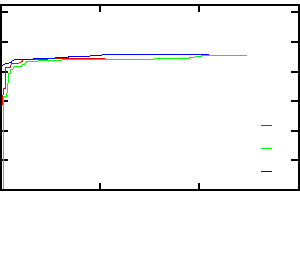
\includegraphics{plot_bubble_fit_l_108_150_combo}}%
    \gplfronttext
  \end{picture}%
\endgroup
}
\caption{Voltage 0.108, 150}
\end{figure}



To test this model, we test it on a single trace obtained at a pressure of \unit{0.108}\volt.
Three runs of the minimisation were taken.  
The initial position and the found minima are displayed in \tabref{plot_bubble_fit_108_150},
and the predicted bubble oscillations are drawn in \figref{plot_bubble_fit_108_150} 

Qualitively, the fits displayed in \figref{plot_bubble_fit_108_150} are convincing.
The fits displayed in \figref{plot_bubble_fit_108_150} have converged to very similar plots.
This can be seen by visual inspection,
but also by examining the log likelihood per data point that is displayed in \figref{plot_bubble_fit_108_150_l:combo}.
The model captures the main features of the experimental data
and has  correctly modelled the  noise so that approximately two thirds of data points are within one-standard-deviation of
the fit.
However, the actual fitted parameters in each plot are very different.
This can be seen in as can be seen by comparing the equilibrium bubble radii.
This suggests that the likelihood is  not a sharply peaked distribution,
and that it might even be multimodal.
This would imply that the estimates for the evidence given in \tabref{plot_bubble_fit_108_150} are unreliable.

%The 
%The likelihood evaluated at each iteration is displayed in \figref{plot_bubble_fit_108_150_l:combo}.
%Although each run took differing number of interations the resultant likelihood was similar in each case.

%\begin{figure}[t]%
%  \centering
%  \subfloat[1st pulse - 1000]{
%    \label{fig:plot_bubble_fit_108_150_p:first}
%    % GNUPLOT: LaTeX picture with Postscript
\begingroup
  \makeatletter
  \providecommand\color[2][]{%
    \GenericError{(gnuplot) \space\space\space\@spaces}{%
      Package color not loaded in conjunction with
      terminal option `colourtext'%
    }{See the gnuplot documentation for explanation.%
    }{Either use 'blacktext' in gnuplot or load the package
      color.sty in LaTeX.}%
    \renewcommand\color[2][]{}%
  }%
  \providecommand\includegraphics[2][]{%
    \GenericError{(gnuplot) \space\space\space\@spaces}{%
      Package graphicx or graphics not loaded%
    }{See the gnuplot documentation for explanation.%
    }{The gnuplot epslatex terminal needs graphicx.sty or graphics.sty.}%
    \renewcommand\includegraphics[2][]{}%
  }%
  \providecommand\rotatebox[2]{#2}%
  \@ifundefined{ifGPcolor}{%
    \newif\ifGPcolor
    \GPcolortrue
  }{}%
  \@ifundefined{ifGPblacktext}{%
    \newif\ifGPblacktext
    \GPblacktexttrue
  }{}%
  % define a \g@addto@macro without @ in the name:
  \let\gplgaddtomacro\g@addto@macro
  % define empty templates for all commands taking text:
  \gdef\gplbacktext{}%
  \gdef\gplfronttext{}%
  \makeatother
  \ifGPblacktext
    % no textcolor at all
    \def\colorrgb#1{}%
    \def\colorgray#1{}%
  \else
    % gray or color?
    \ifGPcolor
      \def\colorrgb#1{\color[rgb]{#1}}%
      \def\colorgray#1{\color[gray]{#1}}%
      \expandafter\def\csname LTw\endcsname{\color{white}}%
      \expandafter\def\csname LTb\endcsname{\color{black}}%
      \expandafter\def\csname LTa\endcsname{\color{black}}%
      \expandafter\def\csname LT0\endcsname{\color[rgb]{1,0,0}}%
      \expandafter\def\csname LT1\endcsname{\color[rgb]{0,1,0}}%
      \expandafter\def\csname LT2\endcsname{\color[rgb]{0,0,1}}%
      \expandafter\def\csname LT3\endcsname{\color[rgb]{1,0,1}}%
      \expandafter\def\csname LT4\endcsname{\color[rgb]{0,1,1}}%
      \expandafter\def\csname LT5\endcsname{\color[rgb]{1,1,0}}%
      \expandafter\def\csname LT6\endcsname{\color[rgb]{0,0,0}}%
      \expandafter\def\csname LT7\endcsname{\color[rgb]{1,0.3,0}}%
      \expandafter\def\csname LT8\endcsname{\color[rgb]{0.5,0.5,0.5}}%
    \else
      % gray
      \def\colorrgb#1{\color{black}}%
      \def\colorgray#1{\color[gray]{#1}}%
      \expandafter\def\csname LTw\endcsname{\color{white}}%
      \expandafter\def\csname LTb\endcsname{\color{black}}%
      \expandafter\def\csname LTa\endcsname{\color{black}}%
      \expandafter\def\csname LT0\endcsname{\color{black}}%
      \expandafter\def\csname LT1\endcsname{\color{black}}%
      \expandafter\def\csname LT2\endcsname{\color{black}}%
      \expandafter\def\csname LT3\endcsname{\color{black}}%
      \expandafter\def\csname LT4\endcsname{\color{black}}%
      \expandafter\def\csname LT5\endcsname{\color{black}}%
      \expandafter\def\csname LT6\endcsname{\color{black}}%
      \expandafter\def\csname LT7\endcsname{\color{black}}%
      \expandafter\def\csname LT8\endcsname{\color{black}}%
    \fi
  \fi
  \setlength{\unitlength}{0.0500bp}%
  \begin{picture}(2880.00,2520.00)%
    \gplgaddtomacro\gplbacktext{%
      \csname LTb\endcsname%
      \put(-119,704){\makebox(0,0)[r]{\strut{}-0.15}}%
      \put(-119,999){\makebox(0,0)[r]{\strut{}-0.1}}%
      \put(-119,1295){\makebox(0,0)[r]{\strut{}-0.05}}%
      \put(-119,1590){\makebox(0,0)[r]{\strut{} 0}}%
      \put(-119,1885){\makebox(0,0)[r]{\strut{} 0.05}}%
      \put(-119,2181){\makebox(0,0)[r]{\strut{} 0.1}}%
      \put(-119,2476){\makebox(0,0)[r]{\strut{} 0.15}}%
      \put(13,484){\makebox(0,0){\strut{} 0}}%
      \put(421,484){\makebox(0,0){\strut{} 5}}%
      \put(828,484){\makebox(0,0){\strut{} 10}}%
      \put(1236,484){\makebox(0,0){\strut{} 15}}%
      \put(1643,484){\makebox(0,0){\strut{} 20}}%
      \put(2051,484){\makebox(0,0){\strut{} 25}}%
      \put(2458,484){\makebox(0,0){\strut{} 30}}%
      \put(2866,484){\makebox(0,0){\strut{} 35}}%
      \put(-1021,1590){\rotatebox{-270}{\makebox(0,0){\footnotesize {Pressure (MPa)}}}}%
      \put(1439,154){\makebox(0,0){\footnotesize {time ($\mu$ s)}}}%
    }%
    \gplgaddtomacro\gplfronttext{%
    }%
    \gplbacktext
    \put(0,0){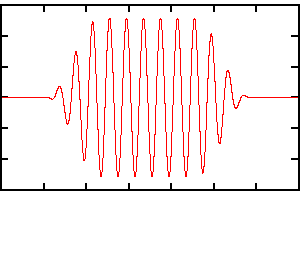
\includegraphics{plot_bubble_fit_p_108_150}}%
    \gplfronttext
  \end{picture}%
\endgroup
}
%\caption{Voltage 0.108, 150}
%\end{figure}


\subsection{Average}

The noise in the first model was too great to be able to say too much.
The noise was too great, which meant that the fits were too permissive.
A large range of models could produce the same results.

To improve the test of the modelling we repeat the same model but this time with the average of 49 alines.
(so that the noise should be reduced by a factor of 7).



\begin{figure}[t]%
  \centering
  \subfloat[1st pulse - 1000]{
    \label{fig::plot_bubble_fit_108_150_av:first}
    % GNUPLOT: LaTeX picture with Postscript
\begingroup
  \makeatletter
  \providecommand\color[2][]{%
    \GenericError{(gnuplot) \space\space\space\@spaces}{%
      Package color not loaded in conjunction with
      terminal option `colourtext'%
    }{See the gnuplot documentation for explanation.%
    }{Either use 'blacktext' in gnuplot or load the package
      color.sty in LaTeX.}%
    \renewcommand\color[2][]{}%
  }%
  \providecommand\includegraphics[2][]{%
    \GenericError{(gnuplot) \space\space\space\@spaces}{%
      Package graphicx or graphics not loaded%
    }{See the gnuplot documentation for explanation.%
    }{The gnuplot epslatex terminal needs graphicx.sty or graphics.sty.}%
    \renewcommand\includegraphics[2][]{}%
  }%
  \providecommand\rotatebox[2]{#2}%
  \@ifundefined{ifGPcolor}{%
    \newif\ifGPcolor
    \GPcolortrue
  }{}%
  \@ifundefined{ifGPblacktext}{%
    \newif\ifGPblacktext
    \GPblacktexttrue
  }{}%
  % define a \g@addto@macro without @ in the name:
  \let\gplgaddtomacro\g@addto@macro
  % define empty templates for all commands taking text:
  \gdef\gplbacktext{}%
  \gdef\gplfronttext{}%
  \makeatother
  \ifGPblacktext
    % no textcolor at all
    \def\colorrgb#1{}%
    \def\colorgray#1{}%
  \else
    % gray or color?
    \ifGPcolor
      \def\colorrgb#1{\color[rgb]{#1}}%
      \def\colorgray#1{\color[gray]{#1}}%
      \expandafter\def\csname LTw\endcsname{\color{white}}%
      \expandafter\def\csname LTb\endcsname{\color{black}}%
      \expandafter\def\csname LTa\endcsname{\color{black}}%
      \expandafter\def\csname LT0\endcsname{\color[rgb]{1,0,0}}%
      \expandafter\def\csname LT1\endcsname{\color[rgb]{0,1,0}}%
      \expandafter\def\csname LT2\endcsname{\color[rgb]{0,0,1}}%
      \expandafter\def\csname LT3\endcsname{\color[rgb]{1,0,1}}%
      \expandafter\def\csname LT4\endcsname{\color[rgb]{0,1,1}}%
      \expandafter\def\csname LT5\endcsname{\color[rgb]{1,1,0}}%
      \expandafter\def\csname LT6\endcsname{\color[rgb]{0,0,0}}%
      \expandafter\def\csname LT7\endcsname{\color[rgb]{1,0.3,0}}%
      \expandafter\def\csname LT8\endcsname{\color[rgb]{0.5,0.5,0.5}}%
    \else
      % gray
      \def\colorrgb#1{\color{black}}%
      \def\colorgray#1{\color[gray]{#1}}%
      \expandafter\def\csname LTw\endcsname{\color{white}}%
      \expandafter\def\csname LTb\endcsname{\color{black}}%
      \expandafter\def\csname LTa\endcsname{\color{black}}%
      \expandafter\def\csname LT0\endcsname{\color{black}}%
      \expandafter\def\csname LT1\endcsname{\color{black}}%
      \expandafter\def\csname LT2\endcsname{\color{black}}%
      \expandafter\def\csname LT3\endcsname{\color{black}}%
      \expandafter\def\csname LT4\endcsname{\color{black}}%
      \expandafter\def\csname LT5\endcsname{\color{black}}%
      \expandafter\def\csname LT6\endcsname{\color{black}}%
      \expandafter\def\csname LT7\endcsname{\color{black}}%
      \expandafter\def\csname LT8\endcsname{\color{black}}%
    \fi
  \fi
  \setlength{\unitlength}{0.0500bp}%
  \begin{picture}(5760.00,2520.00)%
    \gplgaddtomacro\gplbacktext{%
      \csname LTb\endcsname%
      \put(-119,704){\makebox(0,0)[r]{\strut{}-0.6}}%
      \put(-119,957){\makebox(0,0)[r]{\strut{}-0.4}}%
      \put(-119,1210){\makebox(0,0)[r]{\strut{}-0.2}}%
      \put(-119,1463){\makebox(0,0)[r]{\strut{} 0}}%
      \put(-119,1717){\makebox(0,0)[r]{\strut{} 0.2}}%
      \put(-119,1970){\makebox(0,0)[r]{\strut{} 0.4}}%
      \put(-119,2223){\makebox(0,0)[r]{\strut{} 0.6}}%
      \put(-119,2476){\makebox(0,0)[r]{\strut{} 0.8}}%
      \put(13,484){\makebox(0,0){\strut{} 0}}%
      \put(832,484){\makebox(0,0){\strut{} 5}}%
      \put(1651,484){\makebox(0,0){\strut{} 10}}%
      \put(2470,484){\makebox(0,0){\strut{} 15}}%
      \put(3289,484){\makebox(0,0){\strut{} 20}}%
      \put(4108,484){\makebox(0,0){\strut{} 25}}%
      \put(4927,484){\makebox(0,0){\strut{} 30}}%
      \put(5746,484){\makebox(0,0){\strut{} 35}}%
      \put(-889,1590){\rotatebox{-270}{\makebox(0,0){\strut{}voltage (V)}}}%
      \put(2879,154){\makebox(0,0){\strut{}time ($\mu$ s)}}%
    }%
    \gplgaddtomacro\gplfronttext{%
      \csname LTb\endcsname%
      \put(5261,2303){\makebox(0,0){\footnotesize {raw}} }%
      \csname LTb\endcsname%
      \put(5261,2083){\makebox(0,0){\footnotesize {1-$\sigma$}}}%
      \csname LTb\endcsname%
      \put(5261,1863){\makebox(0,0){\footnotesize {fit}}}%
    }%
    \gplbacktext
    \put(0,0){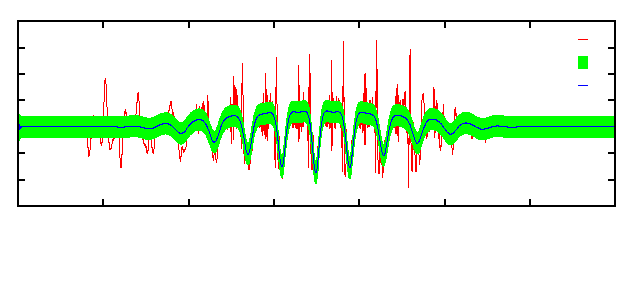
\includegraphics{plot_bubble_fit_108_150_av_b}}%
    \gplfronttext
  \end{picture}%
\endgroup
}
\caption{Voltage 0.108, 150}
\end{figure}

\begin{figure}[t]%
  \centering
  \subfloat[1st pulse - 1000]{
    \label{fig:param_108_150_av_b_likelihood}
    % GNUPLOT: LaTeX picture with Postscript
\begingroup
  \makeatletter
  \providecommand\color[2][]{%
    \GenericError{(gnuplot) \space\space\space\@spaces}{%
      Package color not loaded in conjunction with
      terminal option `colourtext'%
    }{See the gnuplot documentation for explanation.%
    }{Either use 'blacktext' in gnuplot or load the package
      color.sty in LaTeX.}%
    \renewcommand\color[2][]{}%
  }%
  \providecommand\includegraphics[2][]{%
    \GenericError{(gnuplot) \space\space\space\@spaces}{%
      Package graphicx or graphics not loaded%
    }{See the gnuplot documentation for explanation.%
    }{The gnuplot epslatex terminal needs graphicx.sty or graphics.sty.}%
    \renewcommand\includegraphics[2][]{}%
  }%
  \providecommand\rotatebox[2]{#2}%
  \@ifundefined{ifGPcolor}{%
    \newif\ifGPcolor
    \GPcolortrue
  }{}%
  \@ifundefined{ifGPblacktext}{%
    \newif\ifGPblacktext
    \GPblacktexttrue
  }{}%
  % define a \g@addto@macro without @ in the name:
  \let\gplgaddtomacro\g@addto@macro
  % define empty templates for all commands taking text:
  \gdef\gplbacktext{}%
  \gdef\gplfronttext{}%
  \makeatother
  \ifGPblacktext
    % no textcolor at all
    \def\colorrgb#1{}%
    \def\colorgray#1{}%
  \else
    % gray or color?
    \ifGPcolor
      \def\colorrgb#1{\color[rgb]{#1}}%
      \def\colorgray#1{\color[gray]{#1}}%
      \expandafter\def\csname LTw\endcsname{\color{white}}%
      \expandafter\def\csname LTb\endcsname{\color{black}}%
      \expandafter\def\csname LTa\endcsname{\color{black}}%
      \expandafter\def\csname LT0\endcsname{\color[rgb]{1,0,0}}%
      \expandafter\def\csname LT1\endcsname{\color[rgb]{0,1,0}}%
      \expandafter\def\csname LT2\endcsname{\color[rgb]{0,0,1}}%
      \expandafter\def\csname LT3\endcsname{\color[rgb]{1,0,1}}%
      \expandafter\def\csname LT4\endcsname{\color[rgb]{0,1,1}}%
      \expandafter\def\csname LT5\endcsname{\color[rgb]{1,1,0}}%
      \expandafter\def\csname LT6\endcsname{\color[rgb]{0,0,0}}%
      \expandafter\def\csname LT7\endcsname{\color[rgb]{1,0.3,0}}%
      \expandafter\def\csname LT8\endcsname{\color[rgb]{0.5,0.5,0.5}}%
    \else
      % gray
      \def\colorrgb#1{\color{black}}%
      \def\colorgray#1{\color[gray]{#1}}%
      \expandafter\def\csname LTw\endcsname{\color{white}}%
      \expandafter\def\csname LTb\endcsname{\color{black}}%
      \expandafter\def\csname LTa\endcsname{\color{black}}%
      \expandafter\def\csname LT0\endcsname{\color{black}}%
      \expandafter\def\csname LT1\endcsname{\color{black}}%
      \expandafter\def\csname LT2\endcsname{\color{black}}%
      \expandafter\def\csname LT3\endcsname{\color{black}}%
      \expandafter\def\csname LT4\endcsname{\color{black}}%
      \expandafter\def\csname LT5\endcsname{\color{black}}%
      \expandafter\def\csname LT6\endcsname{\color{black}}%
      \expandafter\def\csname LT7\endcsname{\color{black}}%
      \expandafter\def\csname LT8\endcsname{\color{black}}%
    \fi
  \fi
  \setlength{\unitlength}{0.0500bp}%
  \begin{picture}(5760.00,2520.00)%
    \gplgaddtomacro\gplbacktext{%
      \csname LTb\endcsname%
      \put(-119,704){\makebox(0,0)[r]{\strut{}-1}}%
      \put(-119,999){\makebox(0,0)[r]{\strut{}-0.5}}%
      \put(-119,1295){\makebox(0,0)[r]{\strut{} 0}}%
      \put(-119,1590){\makebox(0,0)[r]{\strut{} 0.5}}%
      \put(-119,1885){\makebox(0,0)[r]{\strut{} 1}}%
      \put(-119,2181){\makebox(0,0)[r]{\strut{} 1.5}}%
      \put(-119,2476){\makebox(0,0)[r]{\strut{} 2}}%
      \put(13,484){\makebox(0,0){\strut{} 0}}%
      \put(1446,484){\makebox(0,0){\strut{} 200}}%
      \put(2880,484){\makebox(0,0){\strut{} 400}}%
      \put(4313,484){\makebox(0,0){\strut{} 600}}%
      \put(5746,484){\makebox(0,0){\strut{} 800}}%
      \put(-889,1590){\rotatebox{-270}{\makebox(0,0){\footnotesize{log(likelihood) per datum}}}}%
      \put(2879,154){\makebox(0,0){\strut{}iteration}}%
    }%
    \gplgaddtomacro\gplfronttext{%
    }%
    \gplbacktext
    \put(0,0){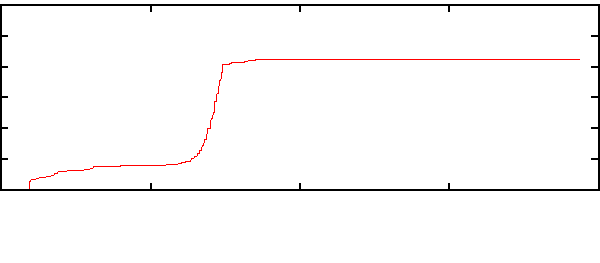
\includegraphics{param_108_150_av_b_likelihood}}%
    \gplfronttext
  \end{picture}%
\endgroup
}\\
  \subfloat[1st pulse - 1000]{
    \label{fig:param_108_150_av_b_rad}
    % GNUPLOT: LaTeX picture with Postscript
\begingroup
  \makeatletter
  \providecommand\color[2][]{%
    \GenericError{(gnuplot) \space\space\space\@spaces}{%
      Package color not loaded in conjunction with
      terminal option `colourtext'%
    }{See the gnuplot documentation for explanation.%
    }{Either use 'blacktext' in gnuplot or load the package
      color.sty in LaTeX.}%
    \renewcommand\color[2][]{}%
  }%
  \providecommand\includegraphics[2][]{%
    \GenericError{(gnuplot) \space\space\space\@spaces}{%
      Package graphicx or graphics not loaded%
    }{See the gnuplot documentation for explanation.%
    }{The gnuplot epslatex terminal needs graphicx.sty or graphics.sty.}%
    \renewcommand\includegraphics[2][]{}%
  }%
  \providecommand\rotatebox[2]{#2}%
  \@ifundefined{ifGPcolor}{%
    \newif\ifGPcolor
    \GPcolortrue
  }{}%
  \@ifundefined{ifGPblacktext}{%
    \newif\ifGPblacktext
    \GPblacktexttrue
  }{}%
  % define a \g@addto@macro without @ in the name:
  \let\gplgaddtomacro\g@addto@macro
  % define empty templates for all commands taking text:
  \gdef\gplbacktext{}%
  \gdef\gplfronttext{}%
  \makeatother
  \ifGPblacktext
    % no textcolor at all
    \def\colorrgb#1{}%
    \def\colorgray#1{}%
  \else
    % gray or color?
    \ifGPcolor
      \def\colorrgb#1{\color[rgb]{#1}}%
      \def\colorgray#1{\color[gray]{#1}}%
      \expandafter\def\csname LTw\endcsname{\color{white}}%
      \expandafter\def\csname LTb\endcsname{\color{black}}%
      \expandafter\def\csname LTa\endcsname{\color{black}}%
      \expandafter\def\csname LT0\endcsname{\color[rgb]{1,0,0}}%
      \expandafter\def\csname LT1\endcsname{\color[rgb]{0,1,0}}%
      \expandafter\def\csname LT2\endcsname{\color[rgb]{0,0,1}}%
      \expandafter\def\csname LT3\endcsname{\color[rgb]{1,0,1}}%
      \expandafter\def\csname LT4\endcsname{\color[rgb]{0,1,1}}%
      \expandafter\def\csname LT5\endcsname{\color[rgb]{1,1,0}}%
      \expandafter\def\csname LT6\endcsname{\color[rgb]{0,0,0}}%
      \expandafter\def\csname LT7\endcsname{\color[rgb]{1,0.3,0}}%
      \expandafter\def\csname LT8\endcsname{\color[rgb]{0.5,0.5,0.5}}%
    \else
      % gray
      \def\colorrgb#1{\color{black}}%
      \def\colorgray#1{\color[gray]{#1}}%
      \expandafter\def\csname LTw\endcsname{\color{white}}%
      \expandafter\def\csname LTb\endcsname{\color{black}}%
      \expandafter\def\csname LTa\endcsname{\color{black}}%
      \expandafter\def\csname LT0\endcsname{\color{black}}%
      \expandafter\def\csname LT1\endcsname{\color{black}}%
      \expandafter\def\csname LT2\endcsname{\color{black}}%
      \expandafter\def\csname LT3\endcsname{\color{black}}%
      \expandafter\def\csname LT4\endcsname{\color{black}}%
      \expandafter\def\csname LT5\endcsname{\color{black}}%
      \expandafter\def\csname LT6\endcsname{\color{black}}%
      \expandafter\def\csname LT7\endcsname{\color{black}}%
      \expandafter\def\csname LT8\endcsname{\color{black}}%
    \fi
  \fi
  \setlength{\unitlength}{0.0500bp}%
  \begin{picture}(5760.00,2520.00)%
    \gplgaddtomacro\gplbacktext{%
      \csname LTb\endcsname%
      \put(-119,704){\makebox(0,0)[r]{\strut{} 0}}%
      \put(-119,1147){\makebox(0,0)[r]{\strut{} 0.5}}%
      \put(-119,1590){\makebox(0,0)[r]{\strut{} 1}}%
      \put(-119,2033){\makebox(0,0)[r]{\strut{} 1.5}}%
      \put(-119,2476){\makebox(0,0)[r]{\strut{} 2}}%
      \put(13,484){\makebox(0,0){\strut{} 0}}%
      \put(1446,484){\makebox(0,0){\strut{} 200}}%
      \put(2880,484){\makebox(0,0){\strut{} 400}}%
      \put(4313,484){\makebox(0,0){\strut{} 600}}%
      \put(5746,484){\makebox(0,0){\strut{} 800}}%
      \put(-889,1590){\rotatebox{-270}{\makebox(0,0){\strut{}radius ($\mu$ m)}}}%
      \put(2879,154){\makebox(0,0){\strut{}iteration}}%
    }%
    \gplgaddtomacro\gplfronttext{%
    }%
    \gplbacktext
    \put(0,0){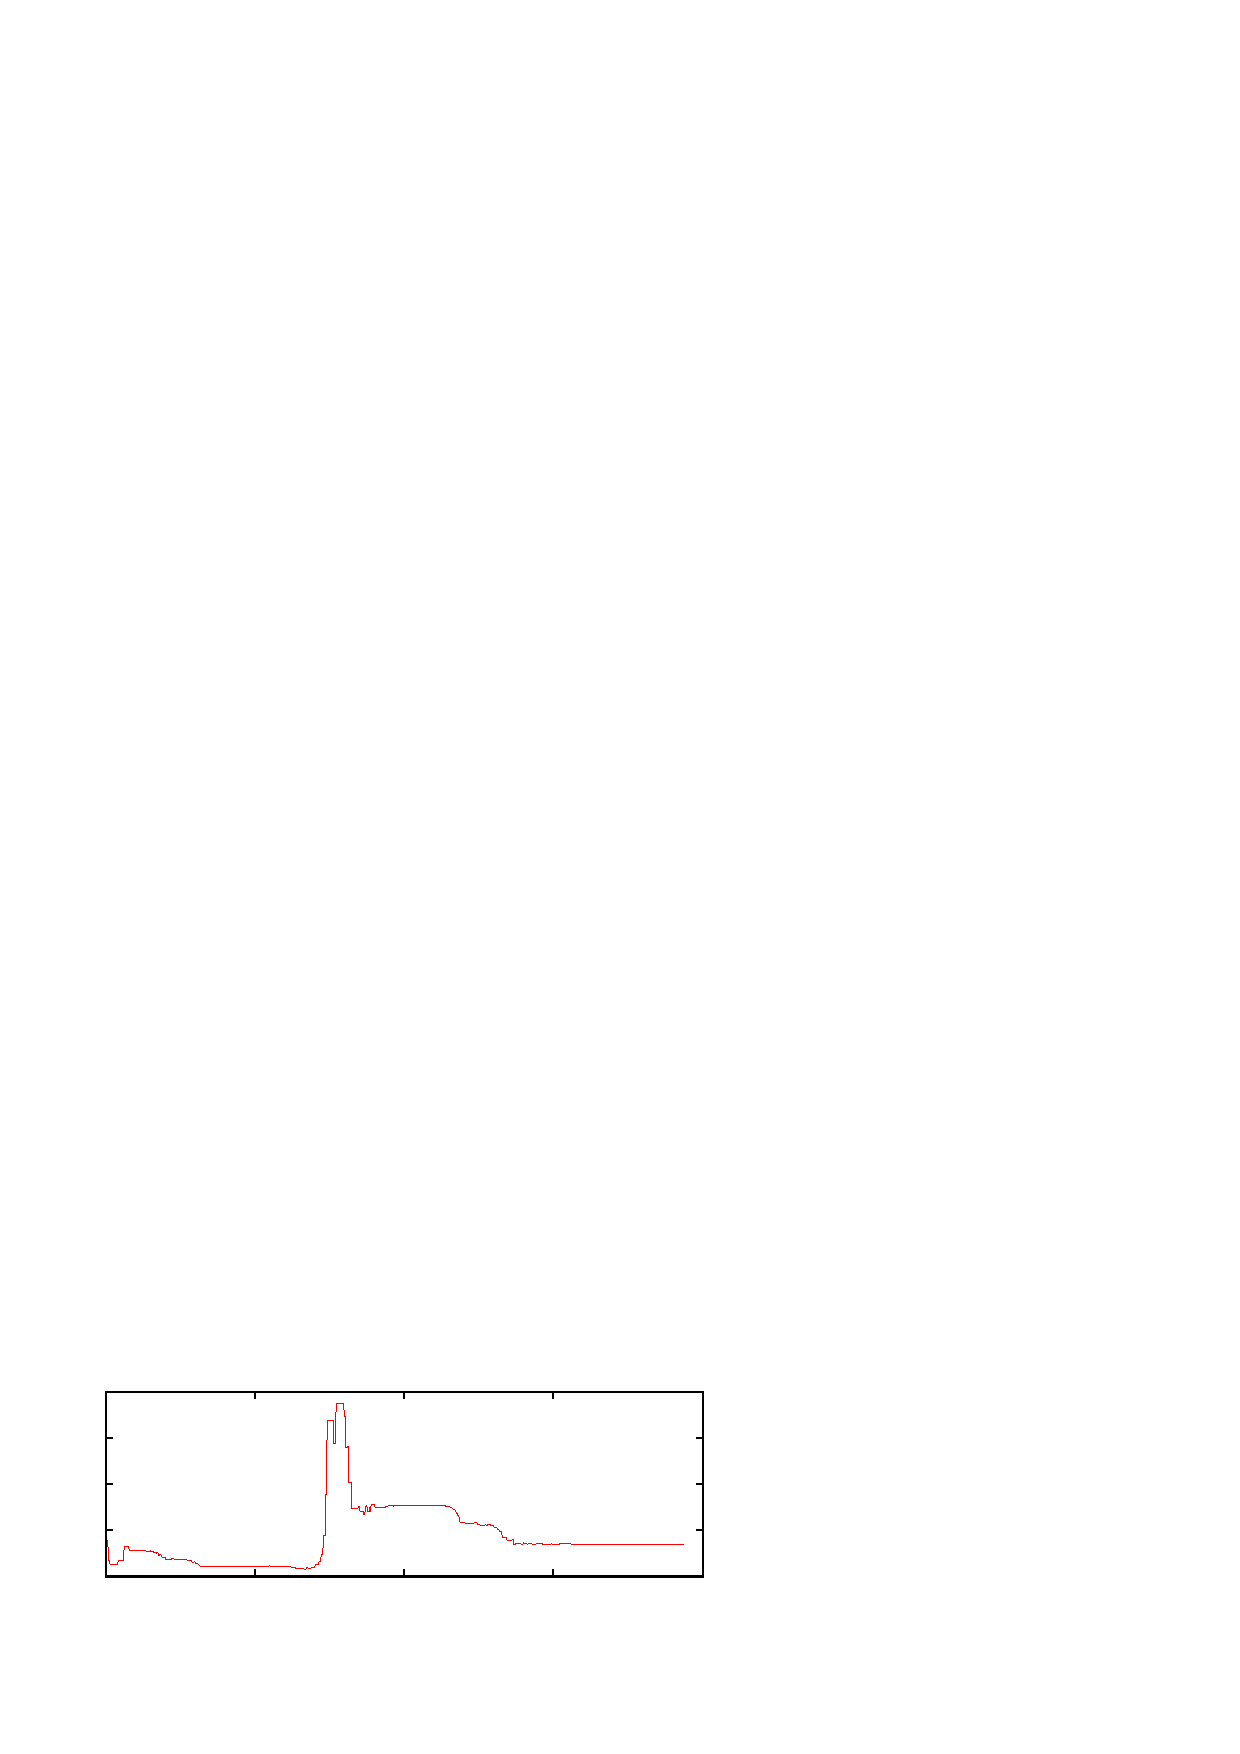
\includegraphics{param_108_150_av_b_rad}}%
    \gplfronttext
  \end{picture}%
\endgroup
}
\caption{Voltage 0.108, 150}
\end{figure}



\ctable[cap     = Parameters for \figref{plot_bubble_fit_108_150:first} (RKM),
        caption = Parameters for \figref{plot_bubble_fit_108_150:first},
        label   = table:plot_bubble_fit_108_150_av_b,
        pos   = h,
        %width = 0.6\textwidth,
        left
       ]
       {llcrccccc}
{
}{\FL
    &   Parameter      &  Initial 1  & Fitted 1   &
    \ML
    &scale factor & 3000 & 1980 &
    \NN
    &standard-deviation & \unit{0.03}\volt & \unit{0.07973}\volt & 
    \NN
    &bubble radius &\unit{0.5}\micro\metre  & \unit{0.3426}\micro\metre& 
    \NN
    &pulse amplitude&\unit{0.1}\mega\pascal &   \unit{0.1357}\mega\pascal &  
    \NN
    &pulse offset &\unit{29.2}\micro\second &   \unit{29.55}\micro\second & 
    \NN
    &pulse tempered ratio &0.5 &1.0 &
    \NN
    &log (evidence) &  &  -11181.21526 &
    \LL
}

The results of the model when fit to the average is displayed in \tabref{plot_bubble_fit_108_150_av_b}
and is drawn in \figref{plot_bubble_fit_108_150_av:first}.
The inferred model is similar to previously,
but in this case, due the increased noise of the experimental data the fitted model is not convincing.
The model does not capture the high frequency detail in the bubble's oscillation,
and this forces the modelled noise to be much greater than it should be.
The reduction in the quality of the fit is indicated by the poor evidence evaluation.
\todo{evaluate evidence comparison}.

Additionally, \figref{param_108_150_av_b_rad} still indicates a problem with metastable states
and converging to differing bubble radii,
even when the likelihood is similar, as is seen in \figref{param_108_150_av_b_likelihood}.


\subsection{Improving the model}
There are a number of improvements that can be made to the model.

\subsubsection{Improving the model of the driving wave}


\begin{figure}[t]%
  \centering
  \subfloat[1st pulse - 1000]{
    \label{fig:plot_bubble_fit_108_150_filter_a:first}
    % GNUPLOT: LaTeX picture with Postscript
\begingroup
  \makeatletter
  \providecommand\color[2][]{%
    \GenericError{(gnuplot) \space\space\space\@spaces}{%
      Package color not loaded in conjunction with
      terminal option `colourtext'%
    }{See the gnuplot documentation for explanation.%
    }{Either use 'blacktext' in gnuplot or load the package
      color.sty in LaTeX.}%
    \renewcommand\color[2][]{}%
  }%
  \providecommand\includegraphics[2][]{%
    \GenericError{(gnuplot) \space\space\space\@spaces}{%
      Package graphicx or graphics not loaded%
    }{See the gnuplot documentation for explanation.%
    }{The gnuplot epslatex terminal needs graphicx.sty or graphics.sty.}%
    \renewcommand\includegraphics[2][]{}%
  }%
  \providecommand\rotatebox[2]{#2}%
  \@ifundefined{ifGPcolor}{%
    \newif\ifGPcolor
    \GPcolortrue
  }{}%
  \@ifundefined{ifGPblacktext}{%
    \newif\ifGPblacktext
    \GPblacktexttrue
  }{}%
  % define a \g@addto@macro without @ in the name:
  \let\gplgaddtomacro\g@addto@macro
  % define empty templates for all commands taking text:
  \gdef\gplbacktext{}%
  \gdef\gplfronttext{}%
  \makeatother
  \ifGPblacktext
    % no textcolor at all
    \def\colorrgb#1{}%
    \def\colorgray#1{}%
  \else
    % gray or color?
    \ifGPcolor
      \def\colorrgb#1{\color[rgb]{#1}}%
      \def\colorgray#1{\color[gray]{#1}}%
      \expandafter\def\csname LTw\endcsname{\color{white}}%
      \expandafter\def\csname LTb\endcsname{\color{black}}%
      \expandafter\def\csname LTa\endcsname{\color{black}}%
      \expandafter\def\csname LT0\endcsname{\color[rgb]{1,0,0}}%
      \expandafter\def\csname LT1\endcsname{\color[rgb]{0,1,0}}%
      \expandafter\def\csname LT2\endcsname{\color[rgb]{0,0,1}}%
      \expandafter\def\csname LT3\endcsname{\color[rgb]{1,0,1}}%
      \expandafter\def\csname LT4\endcsname{\color[rgb]{0,1,1}}%
      \expandafter\def\csname LT5\endcsname{\color[rgb]{1,1,0}}%
      \expandafter\def\csname LT6\endcsname{\color[rgb]{0,0,0}}%
      \expandafter\def\csname LT7\endcsname{\color[rgb]{1,0.3,0}}%
      \expandafter\def\csname LT8\endcsname{\color[rgb]{0.5,0.5,0.5}}%
    \else
      % gray
      \def\colorrgb#1{\color{black}}%
      \def\colorgray#1{\color[gray]{#1}}%
      \expandafter\def\csname LTw\endcsname{\color{white}}%
      \expandafter\def\csname LTb\endcsname{\color{black}}%
      \expandafter\def\csname LTa\endcsname{\color{black}}%
      \expandafter\def\csname LT0\endcsname{\color{black}}%
      \expandafter\def\csname LT1\endcsname{\color{black}}%
      \expandafter\def\csname LT2\endcsname{\color{black}}%
      \expandafter\def\csname LT3\endcsname{\color{black}}%
      \expandafter\def\csname LT4\endcsname{\color{black}}%
      \expandafter\def\csname LT5\endcsname{\color{black}}%
      \expandafter\def\csname LT6\endcsname{\color{black}}%
      \expandafter\def\csname LT7\endcsname{\color{black}}%
      \expandafter\def\csname LT8\endcsname{\color{black}}%
    \fi
  \fi
  \setlength{\unitlength}{0.0500bp}%
  \begin{picture}(5760.00,2520.00)%
    \gplgaddtomacro\gplbacktext{%
      \csname LTb\endcsname%
      \put(-119,704){\makebox(0,0)[r]{\strut{}-0.6}}%
      \put(-119,957){\makebox(0,0)[r]{\strut{}-0.4}}%
      \put(-119,1210){\makebox(0,0)[r]{\strut{}-0.2}}%
      \put(-119,1463){\makebox(0,0)[r]{\strut{} 0}}%
      \put(-119,1717){\makebox(0,0)[r]{\strut{} 0.2}}%
      \put(-119,1970){\makebox(0,0)[r]{\strut{} 0.4}}%
      \put(-119,2223){\makebox(0,0)[r]{\strut{} 0.6}}%
      \put(-119,2476){\makebox(0,0)[r]{\strut{} 0.8}}%
      \put(13,484){\makebox(0,0){\strut{} 0}}%
      \put(832,484){\makebox(0,0){\strut{} 5}}%
      \put(1651,484){\makebox(0,0){\strut{} 10}}%
      \put(2470,484){\makebox(0,0){\strut{} 15}}%
      \put(3289,484){\makebox(0,0){\strut{} 20}}%
      \put(4108,484){\makebox(0,0){\strut{} 25}}%
      \put(4927,484){\makebox(0,0){\strut{} 30}}%
      \put(5746,484){\makebox(0,0){\strut{} 35}}%
      \put(-889,1590){\rotatebox{-270}{\makebox(0,0){\strut{}voltage (V)}}}%
      \put(2879,154){\makebox(0,0){\strut{}time ($\mu$ s)}}%
    }%
    \gplgaddtomacro\gplfronttext{%
      \csname LTb\endcsname%
      \put(5261,2303){\makebox(0,0){\footnotesize {raw}} }%
      \csname LTb\endcsname%
      \put(5261,2083){\makebox(0,0){\footnotesize {1-$\sigma$}}}%
      \csname LTb\endcsname%
      \put(5261,1863){\makebox(0,0){\footnotesize {fit}}}%
    }%
    \gplbacktext
    \put(0,0){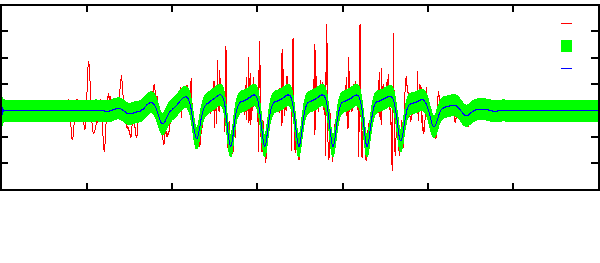
\includegraphics{plot_bubble_fit_108_150_av_2_wave_a}}%
    \gplfronttext
  \end{picture}%
\endgroup
}
\caption{Voltage 0.108, 150 }
\end{figure}


\ctable[cap     = Parameters for \figref{plot_bubble_fit_108_150:first} (RKM),
        caption = Parameters for \figref{plot_bubble_fit_108_150:first},
        label   = table:fit_108_150:first,
        pos   = h,
        %width = 0.6\textwidth,
        left
       ]
       {llcrccccc}
{
}{\FL
    &   Parameter      &  Initial 1  & Fitted 1   &
    \ML
    &scale factor & 3000 & 1980 & 2447 &
    \NN
    &standard-deviation &  \unit{0.07973}\volt &  \unit{0.07910}\volt &
    \NN
    &bubble radius & \unit{0.3426}\micro\metre&  \unit{0.2959}\micro\metre& 
    \NN
    &pulse 1 amplitude& \unit{0.1357}\mega\pascal & \unit{0.1334}\mega\pascal  &
    \NN
    &pulse 1 offset & \unit{29.55}\micro\second & \unit{29.51}\micro\second &
    \NN
    &pulse 1 tempered ratio &0.5 & 0.65021 &
    \NN
    &pulse 2 amplitude& \unit{0.01}\mega\pascal & \unit{0.0070827}\mega\pascal  &
    \NN
    &pulse 2 offset & \unit{29.3}\micro\second & \unit{29.254}\micro\second &
    \NN
    &pulse 2 tempered ratio &0.5 & 0.50386 &
    \NN
    &log (evidence) &  & -11443.50021  &
    \LL
}

\begin{figure}[t]%
  \centering
  \subfloat[1st pulse - 1000]{
    \label{fig:plot_bubble_fit_108_150_filter_a:first}
    % GNUPLOT: LaTeX picture with Postscript
\begingroup
  \makeatletter
  \providecommand\color[2][]{%
    \GenericError{(gnuplot) \space\space\space\@spaces}{%
      Package color not loaded in conjunction with
      terminal option `colourtext'%
    }{See the gnuplot documentation for explanation.%
    }{Either use 'blacktext' in gnuplot or load the package
      color.sty in LaTeX.}%
    \renewcommand\color[2][]{}%
  }%
  \providecommand\includegraphics[2][]{%
    \GenericError{(gnuplot) \space\space\space\@spaces}{%
      Package graphicx or graphics not loaded%
    }{See the gnuplot documentation for explanation.%
    }{The gnuplot epslatex terminal needs graphicx.sty or graphics.sty.}%
    \renewcommand\includegraphics[2][]{}%
  }%
  \providecommand\rotatebox[2]{#2}%
  \@ifundefined{ifGPcolor}{%
    \newif\ifGPcolor
    \GPcolortrue
  }{}%
  \@ifundefined{ifGPblacktext}{%
    \newif\ifGPblacktext
    \GPblacktexttrue
  }{}%
  % define a \g@addto@macro without @ in the name:
  \let\gplgaddtomacro\g@addto@macro
  % define empty templates for all commands taking text:
  \gdef\gplbacktext{}%
  \gdef\gplfronttext{}%
  \makeatother
  \ifGPblacktext
    % no textcolor at all
    \def\colorrgb#1{}%
    \def\colorgray#1{}%
  \else
    % gray or color?
    \ifGPcolor
      \def\colorrgb#1{\color[rgb]{#1}}%
      \def\colorgray#1{\color[gray]{#1}}%
      \expandafter\def\csname LTw\endcsname{\color{white}}%
      \expandafter\def\csname LTb\endcsname{\color{black}}%
      \expandafter\def\csname LTa\endcsname{\color{black}}%
      \expandafter\def\csname LT0\endcsname{\color[rgb]{1,0,0}}%
      \expandafter\def\csname LT1\endcsname{\color[rgb]{0,1,0}}%
      \expandafter\def\csname LT2\endcsname{\color[rgb]{0,0,1}}%
      \expandafter\def\csname LT3\endcsname{\color[rgb]{1,0,1}}%
      \expandafter\def\csname LT4\endcsname{\color[rgb]{0,1,1}}%
      \expandafter\def\csname LT5\endcsname{\color[rgb]{1,1,0}}%
      \expandafter\def\csname LT6\endcsname{\color[rgb]{0,0,0}}%
      \expandafter\def\csname LT7\endcsname{\color[rgb]{1,0.3,0}}%
      \expandafter\def\csname LT8\endcsname{\color[rgb]{0.5,0.5,0.5}}%
    \else
      % gray
      \def\colorrgb#1{\color{black}}%
      \def\colorgray#1{\color[gray]{#1}}%
      \expandafter\def\csname LTw\endcsname{\color{white}}%
      \expandafter\def\csname LTb\endcsname{\color{black}}%
      \expandafter\def\csname LTa\endcsname{\color{black}}%
      \expandafter\def\csname LT0\endcsname{\color{black}}%
      \expandafter\def\csname LT1\endcsname{\color{black}}%
      \expandafter\def\csname LT2\endcsname{\color{black}}%
      \expandafter\def\csname LT3\endcsname{\color{black}}%
      \expandafter\def\csname LT4\endcsname{\color{black}}%
      \expandafter\def\csname LT5\endcsname{\color{black}}%
      \expandafter\def\csname LT6\endcsname{\color{black}}%
      \expandafter\def\csname LT7\endcsname{\color{black}}%
      \expandafter\def\csname LT8\endcsname{\color{black}}%
    \fi
  \fi
  \setlength{\unitlength}{0.0500bp}%
  \begin{picture}(5760.00,2520.00)%
    \gplgaddtomacro\gplbacktext{%
      \csname LTb\endcsname%
      \put(-119,704){\makebox(0,0)[r]{\strut{}-0.6}}%
      \put(-119,957){\makebox(0,0)[r]{\strut{}-0.4}}%
      \put(-119,1210){\makebox(0,0)[r]{\strut{}-0.2}}%
      \put(-119,1463){\makebox(0,0)[r]{\strut{} 0}}%
      \put(-119,1717){\makebox(0,0)[r]{\strut{} 0.2}}%
      \put(-119,1970){\makebox(0,0)[r]{\strut{} 0.4}}%
      \put(-119,2223){\makebox(0,0)[r]{\strut{} 0.6}}%
      \put(-119,2476){\makebox(0,0)[r]{\strut{} 0.8}}%
      \put(13,484){\makebox(0,0){\strut{} 0}}%
      \put(832,484){\makebox(0,0){\strut{} 5}}%
      \put(1651,484){\makebox(0,0){\strut{} 10}}%
      \put(2470,484){\makebox(0,0){\strut{} 15}}%
      \put(3289,484){\makebox(0,0){\strut{} 20}}%
      \put(4108,484){\makebox(0,0){\strut{} 25}}%
      \put(4927,484){\makebox(0,0){\strut{} 30}}%
      \put(5746,484){\makebox(0,0){\strut{} 35}}%
      \put(-889,1590){\rotatebox{-270}{\makebox(0,0){\strut{}voltage (V)}}}%
      \put(2879,154){\makebox(0,0){\strut{}time ($\mu$ s)}}%
    }%
    \gplgaddtomacro\gplfronttext{%
      \csname LTb\endcsname%
      \put(5261,2303){\makebox(0,0){\footnotesize {raw}} }%
      \csname LTb\endcsname%
      \put(5261,2083){\makebox(0,0){\footnotesize {1-$\sigma$}}}%
      \csname LTb\endcsname%
      \put(5261,1863){\makebox(0,0){\footnotesize {fit}}}%
    }%
    \gplbacktext
    \put(0,0){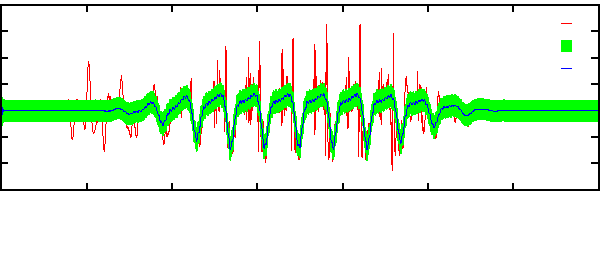
\includegraphics{plot_bubble_fit_108_150_av_3_wave_a}}%
    \gplfronttext
  \end{picture}%
\endgroup
}
\caption{Voltage 0.108, 150 }
\end{figure}

\ctable[cap     = Parameters for \figref{plot_bubble_fit_108_150:first} (RKM),
        caption = Parameters for \figref{plot_bubble_fit_108_150:first},
        label   = table:fit_108_150:first,
        pos   = h,
        %width = 0.6\textwidth,
        left
       ]
       {llcrccccc}
{
}{\FL
    &   Parameter      &  Initial 1  & Fitted 1   &
    \ML
    &scale factor  & 2447 &  2507.1&
    \NN
    &standard-deviation &  \unit{0.07910}\volt &\unit{0.07910}\volt &
    \NN
    &bubble radius &  \unit{0.2959}\micro\metre& \unit{0.2932}\micro\metre &
    \NN
    &pulse 1 amplitude& \unit{0.1334}\mega\pascal  & \unit{0.1295}\mega\pascal&
    \NN
    &pulse 1 offset & \unit{29.51}\micro\second &\unit{29.51}\micro\second &
    \NN
    &pulse 1 tempered ratio & 0.65021 & 0.66728 &
    \NN
    &pulse 2 amplitude& \unit{0.0070827}\mega\pascal  &\unit{0.007957}\mega\pascal  &
    \NN
    &pulse 2 offset &  \unit{29.254}\micro\second &\unit{29.23}\micro\second &
    \NN
    &pulse 2 tempered ratio  & 0.50386 & 0.51508 &  
    \NN
    &pulse 3 frequency & \unit{10.0}\mega\hertz  &\unit{6.1037}\mega\hertz &
    \NN
    &pulse 3 amplitude& \unit{0.0001}\mega\pascal  & \unit{0.007137}\mega\pascal &
    \NN
    &pulse 3 offset &  \unit{29.3}\micro\second &\unit{29.27}\micro\second &
    \NN
    &pulse 3 tempered ratio  & 0.5 &0.74246 &  
    \NN
    &log (evidence) &  &  -11582.22102 &
    \LL
}






Can increase the number of subcomponents of the driving wave.
Then have a set of $n$
\nlist{
  \item amplitude
  \item offset
}
with the frequencies taken as harmonics of the original \unit{0.5}\mega\hertz\ wave.
An illustration is provided in \figref{}.
It is seen that the bubble is really quite sensitive to the driving wave.
The number of parameters increases and the fit imporves,
but from the evidence value it is seen that the quality of the model decreases.
The reason is that the parameters space that can be explored grows faster than 
the improved fitness of the model.




\subsubsection{Modelling the bandwidth}

\begin{figure}[t]%
  \centering
  \subfloat[1st pulse - 1000]{
    \label{fig:plot_bubble_fit_108_150_filter_a:first}
    % GNUPLOT: LaTeX picture with Postscript
\begingroup
  \makeatletter
  \providecommand\color[2][]{%
    \GenericError{(gnuplot) \space\space\space\@spaces}{%
      Package color not loaded in conjunction with
      terminal option `colourtext'%
    }{See the gnuplot documentation for explanation.%
    }{Either use 'blacktext' in gnuplot or load the package
      color.sty in LaTeX.}%
    \renewcommand\color[2][]{}%
  }%
  \providecommand\includegraphics[2][]{%
    \GenericError{(gnuplot) \space\space\space\@spaces}{%
      Package graphicx or graphics not loaded%
    }{See the gnuplot documentation for explanation.%
    }{The gnuplot epslatex terminal needs graphicx.sty or graphics.sty.}%
    \renewcommand\includegraphics[2][]{}%
  }%
  \providecommand\rotatebox[2]{#2}%
  \@ifundefined{ifGPcolor}{%
    \newif\ifGPcolor
    \GPcolortrue
  }{}%
  \@ifundefined{ifGPblacktext}{%
    \newif\ifGPblacktext
    \GPblacktexttrue
  }{}%
  % define a \g@addto@macro without @ in the name:
  \let\gplgaddtomacro\g@addto@macro
  % define empty templates for all commands taking text:
  \gdef\gplbacktext{}%
  \gdef\gplfronttext{}%
  \makeatother
  \ifGPblacktext
    % no textcolor at all
    \def\colorrgb#1{}%
    \def\colorgray#1{}%
  \else
    % gray or color?
    \ifGPcolor
      \def\colorrgb#1{\color[rgb]{#1}}%
      \def\colorgray#1{\color[gray]{#1}}%
      \expandafter\def\csname LTw\endcsname{\color{white}}%
      \expandafter\def\csname LTb\endcsname{\color{black}}%
      \expandafter\def\csname LTa\endcsname{\color{black}}%
      \expandafter\def\csname LT0\endcsname{\color[rgb]{1,0,0}}%
      \expandafter\def\csname LT1\endcsname{\color[rgb]{0,1,0}}%
      \expandafter\def\csname LT2\endcsname{\color[rgb]{0,0,1}}%
      \expandafter\def\csname LT3\endcsname{\color[rgb]{1,0,1}}%
      \expandafter\def\csname LT4\endcsname{\color[rgb]{0,1,1}}%
      \expandafter\def\csname LT5\endcsname{\color[rgb]{1,1,0}}%
      \expandafter\def\csname LT6\endcsname{\color[rgb]{0,0,0}}%
      \expandafter\def\csname LT7\endcsname{\color[rgb]{1,0.3,0}}%
      \expandafter\def\csname LT8\endcsname{\color[rgb]{0.5,0.5,0.5}}%
    \else
      % gray
      \def\colorrgb#1{\color{black}}%
      \def\colorgray#1{\color[gray]{#1}}%
      \expandafter\def\csname LTw\endcsname{\color{white}}%
      \expandafter\def\csname LTb\endcsname{\color{black}}%
      \expandafter\def\csname LTa\endcsname{\color{black}}%
      \expandafter\def\csname LT0\endcsname{\color{black}}%
      \expandafter\def\csname LT1\endcsname{\color{black}}%
      \expandafter\def\csname LT2\endcsname{\color{black}}%
      \expandafter\def\csname LT3\endcsname{\color{black}}%
      \expandafter\def\csname LT4\endcsname{\color{black}}%
      \expandafter\def\csname LT5\endcsname{\color{black}}%
      \expandafter\def\csname LT6\endcsname{\color{black}}%
      \expandafter\def\csname LT7\endcsname{\color{black}}%
      \expandafter\def\csname LT8\endcsname{\color{black}}%
    \fi
  \fi
  \setlength{\unitlength}{0.0500bp}%
  \begin{picture}(5760.00,2520.00)%
    \gplgaddtomacro\gplbacktext{%
      \csname LTb\endcsname%
      \put(-119,704){\makebox(0,0)[r]{\strut{}-0.6}}%
      \put(-119,957){\makebox(0,0)[r]{\strut{}-0.4}}%
      \put(-119,1210){\makebox(0,0)[r]{\strut{}-0.2}}%
      \put(-119,1463){\makebox(0,0)[r]{\strut{} 0}}%
      \put(-119,1717){\makebox(0,0)[r]{\strut{} 0.2}}%
      \put(-119,1970){\makebox(0,0)[r]{\strut{} 0.4}}%
      \put(-119,2223){\makebox(0,0)[r]{\strut{} 0.6}}%
      \put(-119,2476){\makebox(0,0)[r]{\strut{} 0.8}}%
      \put(13,484){\makebox(0,0){\strut{} 0}}%
      \put(832,484){\makebox(0,0){\strut{} 5}}%
      \put(1651,484){\makebox(0,0){\strut{} 10}}%
      \put(2470,484){\makebox(0,0){\strut{} 15}}%
      \put(3289,484){\makebox(0,0){\strut{} 20}}%
      \put(4108,484){\makebox(0,0){\strut{} 25}}%
      \put(4927,484){\makebox(0,0){\strut{} 30}}%
      \put(5746,484){\makebox(0,0){\strut{} 35}}%
      \put(-889,1590){\rotatebox{-270}{\makebox(0,0){\strut{}voltage (V)}}}%
      \put(2879,154){\makebox(0,0){\strut{}time ($\mu$ s)}}%
    }%
    \gplgaddtomacro\gplfronttext{%
      \csname LTb\endcsname%
      \put(5261,2303){\makebox(0,0){\footnotesize {raw}} }%
      \csname LTb\endcsname%
      \put(5261,2083){\makebox(0,0){\footnotesize {1-$\sigma$}}}%
      \csname LTb\endcsname%
      \put(5261,1863){\makebox(0,0){\footnotesize {fit}}}%
    }%
    \gplbacktext
    \put(0,0){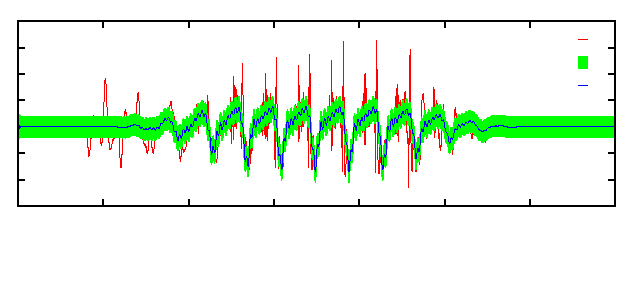
\includegraphics{plot_bubble_fit_108_150_av_3_wave_filter_a}}%
    \gplfronttext
  \end{picture}%
\endgroup
}
\caption{Voltage 0.108, 150 }
\end{figure}

\ctable[cap     = Parameters for \figref{plot_bubble_fit_108_150:first} (RKM),
        caption = Parameters for \figref{plot_bubble_fit_108_150:first},
        label   = table:fit_108_150:first,
        pos   = h,
        %width = 0.6\textwidth,
        left
       ]
       {llcrccccc}
{
}{\FL
    &   Parameter      &  Initial 1  & Fitted 1   &
    \ML
    &scale factor  & 2447 &  3490&
    \NN
    &standard-deviation &  \unit{0.07910}\volt &\unit{0.079354}\volt &
    \NN
    &bubble radius &  \unit{0.2959}\micro\metre& \unit{0.2854}\micro\metre &
    \NN
    &pulse 1 amplitude& \unit{0.1334}\mega\pascal  & \unit{0.15067}\mega\pascal&
    \NN
    &pulse 1 offset & \unit{29.51}\micro\second &\unit{29.48}\micro\second &
    \NN
    &pulse 1 tempered ratio & 0.65021 & 0.69596  &
    \NN
    &pulse 2 amplitude& \unit{0.0070827}\mega\pascal  &\unit{0.014243}\mega\pascal  &
    \NN
    &pulse 2 offset &  \unit{29.254}\micro\second &\unit{29.30}\micro\second &
    \NN
    &pulse 2 tempered ratio  & 0.50386 &  0.66594 &  
    \NN
    &pulse 3 frequency & \unit{10.0}\mega\hertz  &\unit{4.5867}\mega\hertz &
    \NN
    &pulse 3 amplitude& \unit{0.0001}\mega\pascal  & \unit{0.00024382}\mega\pascal &
    \NN
    &pulse 3 offset &  \unit{29.3}\micro\second &\unit{29.12}\micro\second &
    \NN
    &pulse 3 tempered ratio  & 0.5 &0.65243 &  
    \NN
    &Fourier frequency& \unit{20}\mega\hertz  & \unit{18.771}\mega\hertz &
    \NN
    &Fourier variance &  \unit{5}\mega\hertz &\unit{11.389}\mega\hertz  &
    \NN
    &Fourier amplitude  & 1.0 &7.2076e+00 &  
    \NN
    &log (evidence) &  & -11845.16088  &
    \LL
}




% \ctable[cap     = Parameters for \figref{plot_bubble_fit_108_150:first} (RKM),
%         caption = Parameters for \figref{plot_bubble_fit_108_150:first},
%         label   = table:fit_108_150:first,
%         pos   = h,
%         %width = 0.6\textwidth,
%         left
%        ]
%        {llcrccccc}
% {
% }{\FL
%     &   Parameter      &  Initial 1  & Fitted 1   &
%     \ML
%     &scale factor & 3000 & 1980 &
%     \NN
%     &standard-deviation &  \unit{0.07973}\volt & 
%     \NN
%     &bubble radius & \unit{0.3426}\micro\metre& 
%     \NN
%     &pulse amplitude&  \unit{0.1357}\mega\pascal &  
%     \NN
%     &pulse offset &   \unit{29.55}\micro\second & 
%     \NN
%     &pulse tempered ratio &0.5 & &
%     \NN
%     &log (evidence) &  &  -11349.69607&
%     \LL
% }


\begin{figure}[t]%
  \centering
  \subfloat[1st pulse - 1000]{
    \label{fig:plot_bubble_fit_108_150_filter_a:first}
    % GNUPLOT: LaTeX picture with Postscript
\begingroup
  \makeatletter
  \providecommand\color[2][]{%
    \GenericError{(gnuplot) \space\space\space\@spaces}{%
      Package color not loaded in conjunction with
      terminal option `colourtext'%
    }{See the gnuplot documentation for explanation.%
    }{Either use 'blacktext' in gnuplot or load the package
      color.sty in LaTeX.}%
    \renewcommand\color[2][]{}%
  }%
  \providecommand\includegraphics[2][]{%
    \GenericError{(gnuplot) \space\space\space\@spaces}{%
      Package graphicx or graphics not loaded%
    }{See the gnuplot documentation for explanation.%
    }{The gnuplot epslatex terminal needs graphicx.sty or graphics.sty.}%
    \renewcommand\includegraphics[2][]{}%
  }%
  \providecommand\rotatebox[2]{#2}%
  \@ifundefined{ifGPcolor}{%
    \newif\ifGPcolor
    \GPcolortrue
  }{}%
  \@ifundefined{ifGPblacktext}{%
    \newif\ifGPblacktext
    \GPblacktexttrue
  }{}%
  % define a \g@addto@macro without @ in the name:
  \let\gplgaddtomacro\g@addto@macro
  % define empty templates for all commands taking text:
  \gdef\gplbacktext{}%
  \gdef\gplfronttext{}%
  \makeatother
  \ifGPblacktext
    % no textcolor at all
    \def\colorrgb#1{}%
    \def\colorgray#1{}%
  \else
    % gray or color?
    \ifGPcolor
      \def\colorrgb#1{\color[rgb]{#1}}%
      \def\colorgray#1{\color[gray]{#1}}%
      \expandafter\def\csname LTw\endcsname{\color{white}}%
      \expandafter\def\csname LTb\endcsname{\color{black}}%
      \expandafter\def\csname LTa\endcsname{\color{black}}%
      \expandafter\def\csname LT0\endcsname{\color[rgb]{1,0,0}}%
      \expandafter\def\csname LT1\endcsname{\color[rgb]{0,1,0}}%
      \expandafter\def\csname LT2\endcsname{\color[rgb]{0,0,1}}%
      \expandafter\def\csname LT3\endcsname{\color[rgb]{1,0,1}}%
      \expandafter\def\csname LT4\endcsname{\color[rgb]{0,1,1}}%
      \expandafter\def\csname LT5\endcsname{\color[rgb]{1,1,0}}%
      \expandafter\def\csname LT6\endcsname{\color[rgb]{0,0,0}}%
      \expandafter\def\csname LT7\endcsname{\color[rgb]{1,0.3,0}}%
      \expandafter\def\csname LT8\endcsname{\color[rgb]{0.5,0.5,0.5}}%
    \else
      % gray
      \def\colorrgb#1{\color{black}}%
      \def\colorgray#1{\color[gray]{#1}}%
      \expandafter\def\csname LTw\endcsname{\color{white}}%
      \expandafter\def\csname LTb\endcsname{\color{black}}%
      \expandafter\def\csname LTa\endcsname{\color{black}}%
      \expandafter\def\csname LT0\endcsname{\color{black}}%
      \expandafter\def\csname LT1\endcsname{\color{black}}%
      \expandafter\def\csname LT2\endcsname{\color{black}}%
      \expandafter\def\csname LT3\endcsname{\color{black}}%
      \expandafter\def\csname LT4\endcsname{\color{black}}%
      \expandafter\def\csname LT5\endcsname{\color{black}}%
      \expandafter\def\csname LT6\endcsname{\color{black}}%
      \expandafter\def\csname LT7\endcsname{\color{black}}%
      \expandafter\def\csname LT8\endcsname{\color{black}}%
    \fi
  \fi
  \setlength{\unitlength}{0.0500bp}%
  \begin{picture}(5760.00,2520.00)%
    \gplgaddtomacro\gplbacktext{%
      \csname LTb\endcsname%
      \put(-119,704){\makebox(0,0)[r]{\strut{}-0.6}}%
      \put(-119,957){\makebox(0,0)[r]{\strut{}-0.4}}%
      \put(-119,1210){\makebox(0,0)[r]{\strut{}-0.2}}%
      \put(-119,1463){\makebox(0,0)[r]{\strut{} 0}}%
      \put(-119,1717){\makebox(0,0)[r]{\strut{} 0.2}}%
      \put(-119,1970){\makebox(0,0)[r]{\strut{} 0.4}}%
      \put(-119,2223){\makebox(0,0)[r]{\strut{} 0.6}}%
      \put(-119,2476){\makebox(0,0)[r]{\strut{} 0.8}}%
      \put(13,484){\makebox(0,0){\strut{} 0}}%
      \put(832,484){\makebox(0,0){\strut{} 5}}%
      \put(1651,484){\makebox(0,0){\strut{} 10}}%
      \put(2470,484){\makebox(0,0){\strut{} 15}}%
      \put(3289,484){\makebox(0,0){\strut{} 20}}%
      \put(4108,484){\makebox(0,0){\strut{} 25}}%
      \put(4927,484){\makebox(0,0){\strut{} 30}}%
      \put(5746,484){\makebox(0,0){\strut{} 35}}%
      \put(-889,1590){\rotatebox{-270}{\makebox(0,0){\strut{}voltage (V)}}}%
      \put(2879,154){\makebox(0,0){\strut{}time ($\mu$ s)}}%
    }%
    \gplgaddtomacro\gplfronttext{%
      \csname LTb\endcsname%
      \put(5261,2303){\makebox(0,0){\footnotesize {raw}} }%
      \csname LTb\endcsname%
      \put(5261,2083){\makebox(0,0){\footnotesize {1-$\sigma$}}}%
      \csname LTb\endcsname%
      \put(5261,1863){\makebox(0,0){\footnotesize {fit}}}%
    }%
    \gplbacktext
    \put(0,0){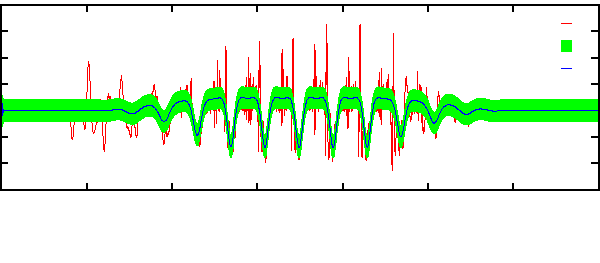
\includegraphics{plot_bubble_fit_108_150_av_filter_a}}%
    \gplfronttext
  \end{picture}%
\endgroup
}
\caption{Voltage 0.108, 150 ln(evidence) = -11349.69607 }
\end{figure}

\begin{figure}[t]%
  \centering
  \subfloat[1st pulse - 1000]{
    \label{fig:plot_bubble_fit_108_150_filter_a:first}
    % GNUPLOT: LaTeX picture with Postscript
\begingroup
  \makeatletter
  \providecommand\color[2][]{%
    \GenericError{(gnuplot) \space\space\space\@spaces}{%
      Package color not loaded in conjunction with
      terminal option `colourtext'%
    }{See the gnuplot documentation for explanation.%
    }{Either use 'blacktext' in gnuplot or load the package
      color.sty in LaTeX.}%
    \renewcommand\color[2][]{}%
  }%
  \providecommand\includegraphics[2][]{%
    \GenericError{(gnuplot) \space\space\space\@spaces}{%
      Package graphicx or graphics not loaded%
    }{See the gnuplot documentation for explanation.%
    }{The gnuplot epslatex terminal needs graphicx.sty or graphics.sty.}%
    \renewcommand\includegraphics[2][]{}%
  }%
  \providecommand\rotatebox[2]{#2}%
  \@ifundefined{ifGPcolor}{%
    \newif\ifGPcolor
    \GPcolortrue
  }{}%
  \@ifundefined{ifGPblacktext}{%
    \newif\ifGPblacktext
    \GPblacktexttrue
  }{}%
  % define a \g@addto@macro without @ in the name:
  \let\gplgaddtomacro\g@addto@macro
  % define empty templates for all commands taking text:
  \gdef\gplbacktext{}%
  \gdef\gplfronttext{}%
  \makeatother
  \ifGPblacktext
    % no textcolor at all
    \def\colorrgb#1{}%
    \def\colorgray#1{}%
  \else
    % gray or color?
    \ifGPcolor
      \def\colorrgb#1{\color[rgb]{#1}}%
      \def\colorgray#1{\color[gray]{#1}}%
      \expandafter\def\csname LTw\endcsname{\color{white}}%
      \expandafter\def\csname LTb\endcsname{\color{black}}%
      \expandafter\def\csname LTa\endcsname{\color{black}}%
      \expandafter\def\csname LT0\endcsname{\color[rgb]{1,0,0}}%
      \expandafter\def\csname LT1\endcsname{\color[rgb]{0,1,0}}%
      \expandafter\def\csname LT2\endcsname{\color[rgb]{0,0,1}}%
      \expandafter\def\csname LT3\endcsname{\color[rgb]{1,0,1}}%
      \expandafter\def\csname LT4\endcsname{\color[rgb]{0,1,1}}%
      \expandafter\def\csname LT5\endcsname{\color[rgb]{1,1,0}}%
      \expandafter\def\csname LT6\endcsname{\color[rgb]{0,0,0}}%
      \expandafter\def\csname LT7\endcsname{\color[rgb]{1,0.3,0}}%
      \expandafter\def\csname LT8\endcsname{\color[rgb]{0.5,0.5,0.5}}%
    \else
      % gray
      \def\colorrgb#1{\color{black}}%
      \def\colorgray#1{\color[gray]{#1}}%
      \expandafter\def\csname LTw\endcsname{\color{white}}%
      \expandafter\def\csname LTb\endcsname{\color{black}}%
      \expandafter\def\csname LTa\endcsname{\color{black}}%
      \expandafter\def\csname LT0\endcsname{\color{black}}%
      \expandafter\def\csname LT1\endcsname{\color{black}}%
      \expandafter\def\csname LT2\endcsname{\color{black}}%
      \expandafter\def\csname LT3\endcsname{\color{black}}%
      \expandafter\def\csname LT4\endcsname{\color{black}}%
      \expandafter\def\csname LT5\endcsname{\color{black}}%
      \expandafter\def\csname LT6\endcsname{\color{black}}%
      \expandafter\def\csname LT7\endcsname{\color{black}}%
      \expandafter\def\csname LT8\endcsname{\color{black}}%
    \fi
  \fi
  \setlength{\unitlength}{0.0500bp}%
  \begin{picture}(5760.00,2520.00)%
    \gplgaddtomacro\gplbacktext{%
      \csname LTb\endcsname%
      \put(-119,704){\makebox(0,0)[r]{\strut{} 0}}%
      \put(-119,957){\makebox(0,0)[r]{\strut{} 0.1}}%
      \put(-119,1210){\makebox(0,0)[r]{\strut{} 0.2}}%
      \put(-119,1463){\makebox(0,0)[r]{\strut{} 0.3}}%
      \put(-119,1717){\makebox(0,0)[r]{\strut{} 0.4}}%
      \put(-119,1970){\makebox(0,0)[r]{\strut{} 0.5}}%
      \put(-119,2223){\makebox(0,0)[r]{\strut{} 0.6}}%
      \put(-119,2476){\makebox(0,0)[r]{\strut{} 0.7}}%
      \put(13,484){\makebox(0,0){\strut{} 0}}%
      \put(969,484){\makebox(0,0){\strut{} 5}}%
      \put(1924,484){\makebox(0,0){\strut{} 10}}%
      \put(2880,484){\makebox(0,0){\strut{} 15}}%
      \put(3835,484){\makebox(0,0){\strut{} 20}}%
      \put(4791,484){\makebox(0,0){\strut{} 25}}%
      \put(5746,484){\makebox(0,0){\strut{} 30}}%
      \put(-889,1590){\rotatebox{-270}{\makebox(0,0){{filter - pass}}}}%
      \put(2879,154){\makebox(0,0){\strut{}frequency (MHz)}}%
    }%
    \gplgaddtomacro\gplfronttext{%
    }%
    \gplbacktext
    \put(0,0){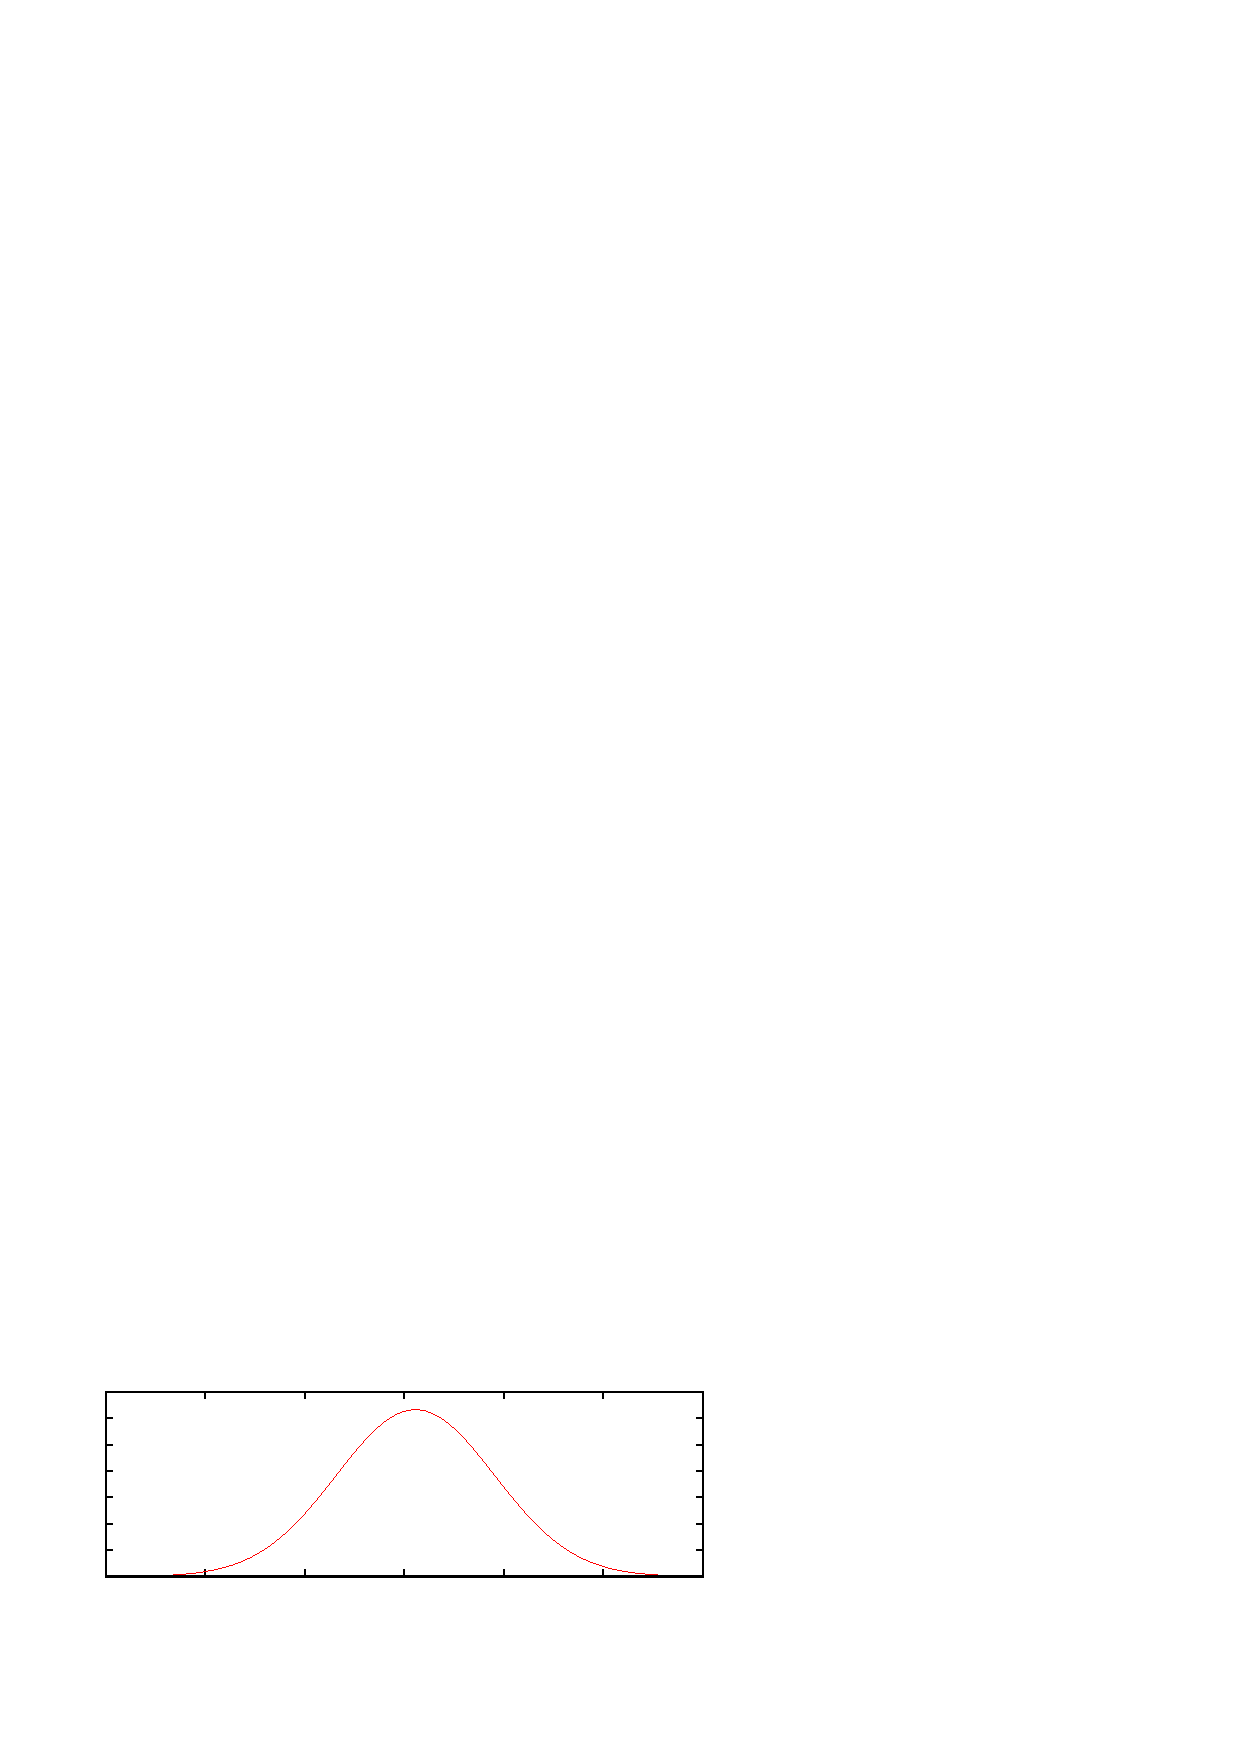
\includegraphics{plot_bubble_fit_108_150_av_filter_a_filter}}%
    \gplfronttext
  \end{picture}%
\endgroup
}
\caption{Voltage 0.108, 150 ln(evidence) = -11349.69607 }
\end{figure}



Firstly,
we can attempt to model the limited bandwidth of the measurements.
We Fourier filter the model with a Gaussian.
The free parameters of this are
\nlist{
  \item central frequency,
  \item amplitude
  \item width
}
The effect of this is shown in \figref{}.



\subsubsection{Multiple bubbles}

The high frequency peaks are not captured with the modelled bubbles so far.
By choosing initial conditions to specifically match these,
we find that the peaks are much greater than are found experimentally.
\Figref{} gives an example.

Can attempt to have multiple bubbles,
one that captures the low frequency bubbles,
one that attempts to capture the high frequency component.

Capturing both is difficult, however. 
The influence of the driving wave is significant on the low frequency part,
and the peaks are a relatively small section of the imaging wave.

To make progress, want to separate the more interesting high frequency component 
from the rest.

Can attempt infer the higher frequency peaks

Problem is that multiple bubbles try to infer the same peaks.
want to separate out the peaks so that different bubbles focus on different aspects
of the image.


\begin{figure}[t]%
  \centering
  \subfloat[1st pulse - 1000]{
    \label{fig:plot_bubble_fit_108_150_filter_a:first}
    % GNUPLOT: LaTeX picture with Postscript
\begingroup
  \makeatletter
  \providecommand\color[2][]{%
    \GenericError{(gnuplot) \space\space\space\@spaces}{%
      Package color not loaded in conjunction with
      terminal option `colourtext'%
    }{See the gnuplot documentation for explanation.%
    }{Either use 'blacktext' in gnuplot or load the package
      color.sty in LaTeX.}%
    \renewcommand\color[2][]{}%
  }%
  \providecommand\includegraphics[2][]{%
    \GenericError{(gnuplot) \space\space\space\@spaces}{%
      Package graphicx or graphics not loaded%
    }{See the gnuplot documentation for explanation.%
    }{The gnuplot epslatex terminal needs graphicx.sty or graphics.sty.}%
    \renewcommand\includegraphics[2][]{}%
  }%
  \providecommand\rotatebox[2]{#2}%
  \@ifundefined{ifGPcolor}{%
    \newif\ifGPcolor
    \GPcolortrue
  }{}%
  \@ifundefined{ifGPblacktext}{%
    \newif\ifGPblacktext
    \GPblacktexttrue
  }{}%
  % define a \g@addto@macro without @ in the name:
  \let\gplgaddtomacro\g@addto@macro
  % define empty templates for all commands taking text:
  \gdef\gplbacktext{}%
  \gdef\gplfronttext{}%
  \makeatother
  \ifGPblacktext
    % no textcolor at all
    \def\colorrgb#1{}%
    \def\colorgray#1{}%
  \else
    % gray or color?
    \ifGPcolor
      \def\colorrgb#1{\color[rgb]{#1}}%
      \def\colorgray#1{\color[gray]{#1}}%
      \expandafter\def\csname LTw\endcsname{\color{white}}%
      \expandafter\def\csname LTb\endcsname{\color{black}}%
      \expandafter\def\csname LTa\endcsname{\color{black}}%
      \expandafter\def\csname LT0\endcsname{\color[rgb]{1,0,0}}%
      \expandafter\def\csname LT1\endcsname{\color[rgb]{0,1,0}}%
      \expandafter\def\csname LT2\endcsname{\color[rgb]{0,0,1}}%
      \expandafter\def\csname LT3\endcsname{\color[rgb]{1,0,1}}%
      \expandafter\def\csname LT4\endcsname{\color[rgb]{0,1,1}}%
      \expandafter\def\csname LT5\endcsname{\color[rgb]{1,1,0}}%
      \expandafter\def\csname LT6\endcsname{\color[rgb]{0,0,0}}%
      \expandafter\def\csname LT7\endcsname{\color[rgb]{1,0.3,0}}%
      \expandafter\def\csname LT8\endcsname{\color[rgb]{0.5,0.5,0.5}}%
    \else
      % gray
      \def\colorrgb#1{\color{black}}%
      \def\colorgray#1{\color[gray]{#1}}%
      \expandafter\def\csname LTw\endcsname{\color{white}}%
      \expandafter\def\csname LTb\endcsname{\color{black}}%
      \expandafter\def\csname LTa\endcsname{\color{black}}%
      \expandafter\def\csname LT0\endcsname{\color{black}}%
      \expandafter\def\csname LT1\endcsname{\color{black}}%
      \expandafter\def\csname LT2\endcsname{\color{black}}%
      \expandafter\def\csname LT3\endcsname{\color{black}}%
      \expandafter\def\csname LT4\endcsname{\color{black}}%
      \expandafter\def\csname LT5\endcsname{\color{black}}%
      \expandafter\def\csname LT6\endcsname{\color{black}}%
      \expandafter\def\csname LT7\endcsname{\color{black}}%
      \expandafter\def\csname LT8\endcsname{\color{black}}%
    \fi
  \fi
  \setlength{\unitlength}{0.0500bp}%
  \begin{picture}(5760.00,2520.00)%
    \gplgaddtomacro\gplbacktext{%
      \csname LTb\endcsname%
      \put(-119,704){\makebox(0,0)[r]{\strut{}-0.6}}%
      \put(-119,957){\makebox(0,0)[r]{\strut{}-0.4}}%
      \put(-119,1210){\makebox(0,0)[r]{\strut{}-0.2}}%
      \put(-119,1463){\makebox(0,0)[r]{\strut{} 0}}%
      \put(-119,1717){\makebox(0,0)[r]{\strut{} 0.2}}%
      \put(-119,1970){\makebox(0,0)[r]{\strut{} 0.4}}%
      \put(-119,2223){\makebox(0,0)[r]{\strut{} 0.6}}%
      \put(-119,2476){\makebox(0,0)[r]{\strut{} 0.8}}%
      \put(13,484){\makebox(0,0){\strut{} 0}}%
      \put(832,484){\makebox(0,0){\strut{} 5}}%
      \put(1651,484){\makebox(0,0){\strut{} 10}}%
      \put(2470,484){\makebox(0,0){\strut{} 15}}%
      \put(3289,484){\makebox(0,0){\strut{} 20}}%
      \put(4108,484){\makebox(0,0){\strut{} 25}}%
      \put(4927,484){\makebox(0,0){\strut{} 30}}%
      \put(5746,484){\makebox(0,0){\strut{} 35}}%
      \put(-889,1590){\rotatebox{-270}{\makebox(0,0){\strut{}voltage (V)}}}%
      \put(2879,154){\makebox(0,0){\strut{}time ($\mu$ s)}}%
    }%
    \gplgaddtomacro\gplfronttext{%
      \csname LTb\endcsname%
      \put(5261,2303){\makebox(0,0){\footnotesize {raw}} }%
      \csname LTb\endcsname%
      \put(5261,2083){\makebox(0,0){\footnotesize {1-$\sigma$}}}%
      \csname LTb\endcsname%
      \put(5261,1863){\makebox(0,0){\footnotesize {fit}}}%
    }%
    \gplbacktext
    \put(0,0){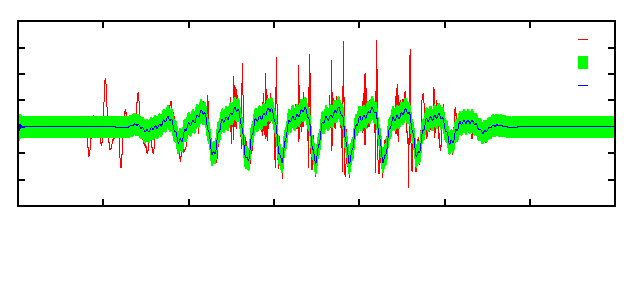
\includegraphics{plot_bubble_fit_108_150_av_3_wave_2_bubble_a}}%
    \gplfronttext
  \end{picture}%
\endgroup
}
\caption{Voltage 0.108, 150}
\end{figure}


\ctable[cap     = Parameters for \figref{plot_bubble_fit_108_150:first} (RKM),
        caption = Parameters for \figref{plot_bubble_fit_108_150:first},
        label   = table:fit_108_150:first,
        pos   = h,
        %width = 0.6\textwidth,
        left
       ]
       {llcrccccc}
{
}{\FL
    &   Parameter      &  Initial 1  & Fitted 1   &
    \ML
    &scale factor  & 2447 & 1868.1 &
    \NN
    &standard-deviation &  \unit{0.07910}\volt &\unit{0.079224}\volt &
    \NN
    &bubble 1 radius &  \unit{0.2959}\micro\metre& \unit{0.41858}\micro\metre &
    \NN
    &bubble 2 radius &  \unit{1.3}\micro\metre& \unit{0.21116}\micro\metre &
    \NN
    &pulse 1 amplitude& \unit{0.1334}\mega\pascal  & \unit{0.062251}\mega\pascal&
    \NN
    &pulse 1 offset & \unit{29.51}\micro\second &\unit{29.51}\micro\second &
    \NN
    &pulse 1 tempered ratio & 0.65021 & 0.65084  &
    \NN
    &pulse 2 amplitude& \unit{0.0070827}\mega\pascal  &\unit{0.0049383}\mega\pascal  &
    \NN
    &pulse 2 offset &  \unit{29.254}\micro\second &\unit{29.165}\micro\second &
    \NN
    &pulse 2 tempered ratio  & 0.50386 & 0.64254  &  
    \NN
    &pulse 3 frequency & \unit{10.0}\mega\hertz  &\unit{4.0901}\mega\hertz &
    \NN
    &pulse 3 amplitude& \unit{0.0001}\mega\pascal  & \unit{0.00010374}\mega\pascal &
    \NN
    &pulse 3 offset &  \unit{29.3}\micro\second &\unit{29.371}\micro\second &
    \NN
    &pulse 3 tempered ratio  & 0.5 &0.36082 &  
    &log (evidence) &  &   -11668.88313 &
    \LL
}

\section{Independent Components of the pulses}

Assume differing bubble sources as independent components in bubble.

\begin{align}
\vx_t = \vA \vs_t
\end{align}
One model for this is a Gaussian
\begin{align}
  P(x_t| \Lambda) = \G(x_t; AS_t, \Lambda)
\end{align}
However,
from the \figref{} it is seen that the Gaussian noise model is not good.
A better alternative is to use Fourier decomposition,

\begin{align}
  \vx_\omega = \vA \vs_\omega
\end{align}
such that
\begin{align}
  P(\vx_\omega| \Lambda_\omega) = \G( \vx_\omega ; AS_\omega, \Lambda_\omega)
\end{align}

\begin{align}
  P(\vH|\vD) = G(\vH)
\end{align}
\begin{align}
\KLD{Q}{P} &= \int_\vH Q(\vH) \log\frac{Q(\vH)}{P(\vH|\vD)} d\vH \\
  &= \int_\vH Q(\vH) \log\frac{Q(\vH)}{P(\vH,\vD)} d\vH  + \int_\vH Q(\vH) \log P(\vD) d\vH\\
  &= \int_\vH Q(\vH) \log Q(\vH) d\vH - \int_\vH Q(\vH) \log Q(\vH) \log P(\vH,\vD) ) d\vH + \log P(\vD)
\end{align}
Bring cost function
\begin{align}
  \L =  \int_\vH Q(\vH) \log Q(\vH) \log P(\vH,\vD) ) d\vH - Q(\vH) \log Q(\vH) d\vH 
\end{align}
From which it follows that
\begin{align}
  \L &=   \log P(\vD,\H) - \KLD{Q}{P} \\
     &\le \log P(\vD,\H)
\end{align}
The probability of the model is 
\begin{align}
  P(\H, \vD) &=    \frac{P(\vD, \H) P(\H)}{P(\vD)}
             &\le  \frac{\L(Q)P(\H)}{P(\vD)}
\end{align}


\subsubsection{The model}
\begin{align}
  P(s_{m\omega}| \H) &= \sum_{c=1}^{N_c} \pi_{mc}\G(s_{m\omega};0,\beta_{\omega c})\\
  P(\beta_{\omega c} &= \GammaDistr(\beta_{mc} ; b^{(\beta)}, c^{(\beta)})\\
  P(\{\pi_{mc}\}_{c=1}^{N_c}|\H)  &= \Dirichlet\lr{ \{\pi_{mc}\}_{c=1}^{N_c} | c^{(\pi)}}
\end{align}
And mixture
\begin{align}
  P(A_{nm}|\H) &= \G(A_{nm}; 0,\alpha_m)\\
  P(\alpha_m| \H) &= \GammaDistr(\alpha_m| b^{(\alpha)},c^{(alpha)})
\end{align}
and gamma
\begin{align}
  P(\Lambda_{\omega},\H) = \GammaDistr(\Lambda_\omega;b^{(\Lambda)},c^{(\Lambda)} )
\end{align}

Simplify the distribution
\begin{align}
Q\lr{\vs, \vA, \pi, \beta, \alpha, \Lambda} = Q\lr{s_{\omega m}}Q\lr{A_{nm}}Q\lr{\pi}Q\lr{\beta}Q\lr{\alpha}Q\lr{\Lambda}
\end{align}

\begin{align}
  Q\lr{s_{nm}} = \G(s_{m \omega};\hat{s}_{m\omega}, \tilde{s}_{m\omega})\\
  Q\lr{A_{nm}} = \G(A_{mn};\hat{A}_{mn}, \tilde{A}_{mn})\\
  Q\lr{\beta_{mc}} = \Gamma(\beta_{mc};\hat{A}_{mn}, \tilde{A}_{mn})
\end{align}


\section{Inferred }


%%% Local Variables: 
%%% mode: latex
%%% TeX-master: "tshorrock_thesis"
%%% End: 